\documentclass[twoside]{mgr}

\usepackage[utf8]{inputenc}
\usepackage[T1]{fontenc}

\usepackage{graphicx}
%\usepackage{subfigure}
\usepackage{subcaption}
\usepackage{caption}
\usepackage{psfrag}
\usepackage{rotating}


\usepackage{amsmath}
\usepackage{amsfonts}
\usepackage{amsthm}
\usepackage{breqn}

\usepackage{supertabular}
\usepackage{array}
\usepackage{tabularx}
\usepackage{hhline}

%\usepackage{showlabels} %dodaje z~boku etykiety

\newtheorem{theorem}{Twierdzenie}[section]
\theoremstyle{definition}
\newtheorem{definition}{Definicja}[section]

\newcommand{\ud}{\mathrm{d}}
\newcommand{\rot}{\mathrm{Rot}}
\newcommand{\tr}{\mathrm{Trans}}

\title{Control algorithms of a skid-steering mobile robot}
\engtitle{Algorytmy sterowania robota mobilnego poruszającego się z poślizgami}
\author{Paweł Bogner}
\supervisor{prof. dr hab. inż. Krzysztof Tchoń, I-6}

\field{Automatyka~i~Robotyka~(AIR)}
\specialisation{Robotyka~(ARR)}

\begin{document}
\maketitle

\tableofcontents

\chapter{Introduction}
The problem of control of skid-steering mobile robots is a very complex issue. 
The main difficulty is to create an adequate model the phenomenon of friciton. 
The authors of \cite{caracciolo1999trajectory} use the Coulomb friction model limited to the low velocities.
Apart from that, the longitudinal skid was neglected. The approach presented in this paper is different.
The assumption is that the skids are possible in both directions, lateral and longitudinal.
This is similar to the models used in automotive literature \cite{pacejka2005tyre}.
All slips are allowed, but the impact of them to the model may be suppressed by tuning the
parameters properly. 

When it comes to the friction model idea, it is based on the velocity of the slip derived
from the Pfaffian matrix. %TODO cite 
Two types of models have been considered here: the linear and the discontinuous model.
The linear friction force model is analogous to the mass on the spring. In that case the friciton
force is proportional to the value of the slip, like the spring reaction force is proportional
to the displacement from the equilibrium position. The second model idea bases on the first one
but includes a modification in order to reflect the fact of losing the traction. Such change
consists in switching the friction coefficient dependently on the value on the slip.

Such systems may be considered on two levels --- kinematic and dynamic. The kinematic model may be
derived basing on the 

Motion planning plays an important part in robot control. This is usually the first step of solving
a certain problem. It is not enough to use a good control algorithm for path following. The fundamental
issue is determining the path or the trajectory to follow. There are many motion planning methods,
such as steering using sinusoid for chained systems \cite{murray1993nonholonomic} or rapidly-exploring random trees for nonholomic systems
with obstacles on the scene \cite{lavalle2000rapidly}. The planning algorithm presented in this paper,
the endogenous configuration approach, can be applied for mobile manipulators, regarding the
mobile platform on dynamic level and the kinematics of the manipulator arm.

The layout of this paper is as follows. Chapter \ref{ch:model} presents the models of researched
objects: the unicycle and RobRex mobile manipulator. Chapter \ref{ch:endogen} introduces the endogenous
configuration space approach to motion planning problem. In chapter \ref{ch:simul}, there are collected
the results of the simulations of the objects mentioned above with application of the motion
planning algorithm. Chapter \ref{ch:concl} summarizes the whole research made.

T\chapter{Model}
In this thesis two different models will be taken into consideration: the unicycle model with system dynamics and RobRex mobile manipulator with platform dynamics and arm kinematics.
\section{Unicycle}


\section{RobRex mobile manipulator}
The model consists of two parts: a mobile platform and a manipulator. The cart has got four fixed-axis wheels, which are actuated with two motors --- the wheels on both sides are coupled. The schematic structure of the vehicle is shown in . %TODO
The manipulator is mounted on the platform above the middle of the front wheel axis.
\subsection{Mobile platform}
Let $w\in \mathbb{R}^5$ be the configuration of the platform, where
$w=(x, y, a\phi, R\theta_1, R\theta_2)$.  
The dynamics model of the cart is analysed in the standard form used in robotics:
\begin{equation}
\label{eq:std_mdl}
P(w)\ddot w + D(w, \dot w) = F(w, \dot w) + Bu.
\end{equation}
The elaborate model derivation can be found in \cite{coupled}. 
The elements of \eqref{eq:std_mdl} are equal to
\begin{align*}
P(w) &= \begin{bmatrix}
Q_{11} & 0 & \frac{Q_{13}}{a} & 0 & 0\\
0 & Q_{22} & \frac{Q_{23}}{a} & 0 & 0\\
\frac{Q_{13}}{a} & \frac{Q_{23}}{a} & \frac{Q_{33}}{a} & 0 & 0\\
0 & 0 & 0 & \frac{Q_{44}}{R^2} & 0 \\
0 & 0 & 0 & 0 & \frac{Q_{55}}{R^2}
\end{bmatrix}, & 
D(w, \dot w) &= \frac{\dot w_3^2}{a^2}\begin{pmatrix}
-Q_{23} & Q_{13} & 0 & 0 & 0
\end{pmatrix}^T
\end{align*}
The components in the above equations are
\begin{align*}
Q_{11} = Q_{22} &= m_p+4m_w,\\
Q_{44} = Q_{55} &= 2I_{w33},\\
Q_{13} &= -m_p(a_{p1}\sin\frac{w_3}{a}+a_{p2}\cos\frac{w_3}{a})- 2m_wa\sin\frac{w_3}{a},\\
Q_{23} &=  m_p(a_{p1}\cos\frac{w_3}{a}-a_{p2}\sin\frac{w_3}{a})+ 2m_wa\cos\frac{w_3}{a},\\
Q_{33} &= I_{p33}+m_p(a_{p1}^2+a_{p2}^2)+4(I_{w11}+m_wb^2)+2m_wa^2.
\end{align*}

The meanings of used symbols are:
\begin{itemize}
\item $m_p$ ---platform mass;
\item $m_w$ ---one wheel mass;
\item $a_{p1}$, $a_{p2}$ --- coordinates of the platform's centre of mass with respect to the platform's coordinate system;
\item $I_{w11}$ --- wheel's moment of inertia with respect to X axis;
\item $I_{w33}$ --- wheel's moment of inertia with respect to Z axis;
\item $I_{p33}$ --- platform's moment of inertia with respect to Z axis.

\end{itemize}

Motion limitations of the platform may be written in Pfaffian form which is 
\begin{equation*}
H(w)=\begin{bmatrix}
-\sin\frac{w_3}{a} & \cos\frac{w_3}{a} & 0 & 0 & 0\\
-\sin\frac{w_3}{a} & \cos\frac{w_3}{a} & 1 & 0 & 0\\
 \cos\frac{w_3}{a} & \sin\frac{w_3}{a} & -\frac{b}{a} & -1 & 0\\
 \cos\frac{w_3}{a} & \sin\frac{w_3}{a} &  \frac{b}{a} &  0 & 1
\end{bmatrix} = \begin{bmatrix}
H^1(w)\\
H^2(w)\\
H^3(w)\\
H^4(w)
\end{bmatrix},
\end{equation*}
where $H^1$ corresponds to the lateral slip of front wheels, $H^2$ to the lateral slip of rear wheel, $H^3$ and $H^4$ depict the longitudinal slips of left and right wheels respectively.



\subsection{Manipulator arm}
The manipulator has got five rotational joints. Its structure is shown in. %TODO
Let $q\in \mathbb{R}^5$ denote the configuration of the arm and $a_2, \dots, a_5$ the lengths of the links. The individual transformation matrices in Denavit-Hartenberg convention are as follows:
\begin{align*}
A_0^1 &= \rot(Z, q_1)\rot(X, \frac{\pi}{2}),\\
A_1^2 &= \rot(Z, q_2)\tr (X, a_2)\rot(X, -\frac{\pi}{2}),\\
A_2^3 &= \rot(Z, q_3)\tr (X, a_3)\rot(X, \frac{\pi}{2}),\\
A_3^4 &= \rot(Z, q_4)\tr (X, a_4)\rot(X, -\frac{\pi}{2}),\\
A_4^5 &= \rot(Z, q_5)\tr (X, a_5).
\end{align*}
In order to reduce kinematics complexity and ease obtaining output function in Euler angles form it has been assumed that third joint is fixed to $0$. This results in the transformation matrix $
A_0^5=\begin{bmatrix}
R_0^5 & T_0^5\\
0 & 1
\end{bmatrix}$, 
where
\begin{align*}
T_0^5 &= \begin{pmatrix}
c_1\left((a_2+a_3)c_2 + c_{24}(a_4+a_5c_5)\right) - a_5s_1s_5\\
s_1\left((a_2+a_3)c_2 + c_{24}(a_4+a_5c_5)\right) + a_5c_1s_5\\
    (a_2+a_3)s_2 + s_{24}(a_4+a_5c_5)
\end{pmatrix},\\
R_0^5 &= \begin{bmatrix}
c_1c_{24}c_5-s_1s_5 & -s_1c_5-c_1c_{24}s_5 & -c_1s_{24}\\
s_1c_{24}c_5-c_1s_5 &  c_1c_5-s_1c_{24}s_5 & -s_1s_{24}\\
s_{24}c_5           & -s_{24}s_5           &  c_{24}
\end{bmatrix}.
\end{align*}
End effector orientation Euler angles (using $\rot(Z,\phi)\rot(X, \theta)\rot(Z, \psi)$) are: $\phi=q_1-\frac{\pi}{2}$, $\theta=q_2+q_4$, $\psi=q_5+\frac{\pi}{2}$.



\chapter{Endogenous configuration space}
Let us consider a mobile robot --- a mobile platform with a manipulator. Let $q \in \mathbb{R}^n$ denote the state of the platform and $x \in \mathbb{R}^p$ denote the configuration of the manipulator. Now we can define a vector $y \in \mathbb{R}^r$ which is the result of the output function $k: \mathbb{R}^n \times \mathbb{R}^p \rightarrow \mathbb{R}^r$. The whole system may be described by the following set of equations:
\begin{align}
\label{eq:control_sys}
\dot q &= f(q) + G(q)u,\\
y &= k(q, x).
\end{align}
This leads to an affine control system with control inputs $u \in \mathbb{R}^m$, $x \in \mathbb{R}^p$ and output function $k$. 

Define a pair $(u(\cdot), x)$, which consists of control inputs mentioned above. Such elements belong to the endogenous configuration space $\mathcal{X} = L_m^2[0, T] \times \mathbb{R}^p$ of the mobile manipulator. The inner product in $\mathcal{X}$ is as follows \cite{ecs_ijc}:
\begin{equation}
\langle (u_1(\cdot), x_1), (u_2(\cdot), x_2) \rangle = \int_0^T u_1^T(t) u_2(t) \ud t + x_1^T x_2.
\end{equation}

This concept can be used in motion planning. The kinematics $K_{q_0, T}: \mathcal{X} \rightarrow \mathbb{R}^r$ allow to determine the state of the mobile manipulator at time $T$ given endogenous configuration $(u(\cdot), x)$ and initial state $q_0$:
\begin{equation}
K_{q_0, T}((u(\cdot), x)) = y(T) = k(\phi_{q_0, T}(u(\cdot)), x),
\end{equation}
where $\phi_{q_0, T}(u(\cdot))$ denotes the flow of the system \eqref{eq:control_sys} caused by input $u(\cdot)$.

With the above definitions the analytic Jacobian can be defined at $(u(\cdot), x) \in \mathcal{X}$:
\begin{align}
J_{q_0, T}(u(\cdot), x)(v(\cdot), w) &= \left.\frac{\ud}{\ud \alpha}\right|_{\alpha=0} K_{q_0, T}((u(\cdot)+\alpha v(\cdot), x+\alpha w))\\
 &= C(T,x)\int_0^T \Phi(T,s)B(s)v(s)\ud s + D(T,x)w,
\end{align}
where $(v(\cdot), w)\in \mathcal{X}$ and $\Phi(T,s)$ is the fundamental matrix of the following system:
\begin{equation}
\begin{aligned}
\label{eq:abxi}
\dot \xi &= A(t)\xi + B(t) v \\
\eta &= C(t)\xi + D(t).
\end{aligned}
\end{equation}
The matrices in \eqref{eq:abxi} are as follows:
\begin{equation}
\begin{aligned}
A(t) &= \frac{\partial (f(q)+G(q)u}{\partial q}, & B(t) &= G(q(t)),\\
C(t) &= \frac{\partial k(q, x)}{\partial q}, & D(t) &= \frac{\partial k(q, x)}{\partial x}.
\end{aligned}
\end{equation}

\section{Computations}
The dimension of $L^2[0,T]$ space is infinite. Therefore we need an infinite number of parameters to define an element from this space. This is impossible to achieve in calculations made on a computer. The solution is to limit the bandwidth of considered functions. 

It is possible to choose a finite-dimensional base $\Phi = [ \phi_1, \phi_2, \dots, \phi_s ]$ spanning the limited-band control functions space. 
With such approach a function $u_i$ is represented by a vector 
$\lambda_i = [\lambda_{i1}, \lambda_{i2}, \dots, \lambda_{is}]^T$ 
which satisfies the formula $u_i = \sum_{k=1}^s \phi_k \lambda_{ik}$.

In order to define a vector $u=[u_1, u_2, \dots, u_m]^T$ a matrix $P(t)$ should be defined, such that $u(t)=P(t)\lambda$. This means $P(t)$ is a block diagonal matrix 
\begin{equation}
P(t)=\begin{bmatrix}
\Phi & 0 & \cdots & 0\\
0 & \Phi & \ddots & \vdots\\
\vdots & \ddots & \ddots & 0 \\
0 &  \cdots & 0 & \Phi
\end{bmatrix}
\end{equation}

Assuming the above the Jacobian $J_{q_0, T}(u(\cdot), x)$ may be computed as $\begin{bmatrix}
C\cdot\Xi(T)& D
\end{bmatrix}$, where $\Xi$ is defined by an ODE $\dot \Xi = A(t)\Xi +B(t)P(t)$ with the initial condition $\Xi(0)=0$ [TODO: citation needed]. This allows easily calculate the Jacobian during the simulation of the system by extending the ODE function.


\chapter{Simulations}
\label{ch:simul}
This chapter presents the results obtained by simulations. The research has been made for two models
described in chapter \ref{ch:model}. The motion planning problem has been solved using endogenous
configuration space approach presented in chapter \ref{ch:endogen}.

There are some issues that are common regardless the studied object. Moreover,
both RobRex mobile manipulator and unicycle have two control inputs. That is why
the same control functions representation may be used in those two models.
The base used to represent the control functions was trigonometric, including up to the third order
harmonics
for the Rex platform
\begin{equation}
\Psi=\begin{pmatrix}
1 & \sin(\omega t) & \cos(\omega t)& \sin(2\omega t) & \cos(2\omega t)& \sin(3\omega t) & \cos(3\omega t)
\end{pmatrix},
\end{equation}
and only with first order harmonics for the unicycle
\begin{equation}
\Psi=\begin{pmatrix}
1 & \sin(\omega t) & \cos(\omega t)
\end{pmatrix},
\end{equation}
where $\omega=\frac{2\pi}{T}$ and $T$ is the control horizon. Assuming the above and
the fact that the models are controlled by two inputs, the
matrix $P(t)$ in \eqref{eq:Pt} is of the form
\begin{equation}
P(t)=\begin{bmatrix}
\Psi & 0\\
0 & \Psi
\end{bmatrix}.
\end{equation}
The decay rate $\gamma$ in \eqref{eq:endogen_num} has been set to $0.05$ for all
the simulations demonstrated in this chapter.

\section{Event mechanism}
In this chapter discontinuous models of a unicycle and mobile platform Rex will be
considered. This induces problems with ODE solving
due to a huge step size contraction in the surroundings of the discontinuities which may
make the computations even impossible to finish. Therefore, an ordinary ODE solving
schema will not perform well in such case.

A solution is to use the event mechanism implemented in MATLAB \cite{events}.
This technique is designed for solving the initial value problems with unknown time of
the end of the simulation. In order to determine when the calculations should end,
we need to define an event function. The event occurs when the event function value
crosses zero. It may be distinguished, if the crossing was in the positive or the negative direction.
Occurring the event may imply calculations termination. 

The event function may be a vector function, i.e. many types of events can be defined. After catching
an event, full information about it may be retrieved: the type of the event, the moment of occurrence,
and the state of the system being simulated. This feature prompts us to use the event mechanism
to simulate discontinuous models.

The idea is quite simple. We define events so that they occur in discontinuities of the
functions defining the simulated model. After catching
an event we stop simulation, save the system state, switch the model, and start new
calculations with the initial state equal to the terminal one from the previous iteration.
In this way a discontinuous system can by simulated easily, avoiding any problems that would
arise using the ordinary approach. Such a concept has been used in calculations presented below.


\section{Unicycle}
The model of a unicycle has been implemented in order to examine the behaviour
of the motion planning algorithm for a very simple object with discontinuities.
The presented model is discontinuous because of the friction coefficients
which are switched according to the slip values.

\subsection{Problem formulation}
The motion planning problem to be solved is kind of a parking manoeuvre. The initial
state of the object is $q_0 = (w_0, \dot{w_0})^T = (0, 0, R\frac{\pi}{2}, 0_5)^T$
and the desired end configuration is $(x, y, \theta) = (10, 0, a\frac{\pi}{2})$.
The motion is supposed to be executed within a fixed control horizon $T$.

\subsection{Simulation conditions}
\label{sec:discont_params_uni}
The parameters of the object used during the simulation are:
\begin{multicols}{2}
\begin{itemize}
\item $m=2 \,\mathrm{kg}$,
\item $R=0.3 \,\mathrm{m}$,
\item $I_\phi =0.045\,\mathrm{kgm^2}$,
\item $I_\theta =0.09\,\mathrm{kgm^2}$. 
\end{itemize}
\end{multicols}
Initial conditions for $\lambda$ parameters used to compute control functions
in \eqref{eq:endogen_num} are
\begin{equation}
\lambda_0=
(\underbrace{0.01, \ 0.001, \ 0.001,}_{u_1}\ \underbrace{0.0001, \ 0, \ 0, \ 0}_{u_2})^T.
\end{equation}
Such setting tries to move the object in the proper direction in the first iteration, in order to
maximise the chances for the algorithm to converge.

The values of the friction coefficients were changing according to the value of the slips $s_\parallel$
and $s_\perp$. 
The point of such an approach is to model the phenomenon
of losing the traction. We will assume that for every friction force we have two
values of the friction coefficient possible: high when the slip is less than the certain
value (traction) and low otherwise (slip). This idea leads to the following formulae
\begin{equation*}
\begin{aligned}
\epsilon&=\begin{cases}
\epsilon_{high} &\mbox{if } |s_\perp| \leq d \\
\epsilon_{low} &\mbox{if } |s_\perp| > d
\end{cases}, &
\tau&=\begin{cases}
\tau_{high} &\mbox{if } |s_\parallel| \leq d \\
\tau_{low} &\mbox{if } |s_\parallel| > d
\end{cases}.
\end{aligned}
\end{equation*}
The values in above equations were set as follows: $\epsilon_{high}=1$, $\epsilon_{low}=0.5$,
$\tau_{high}=10$, $\tau_{low}=0.3$, $d=0.15$. The characteristics of the friction is depicted
in figure \ref{fig:fric}.
\begin{figure}[htb]
\centering
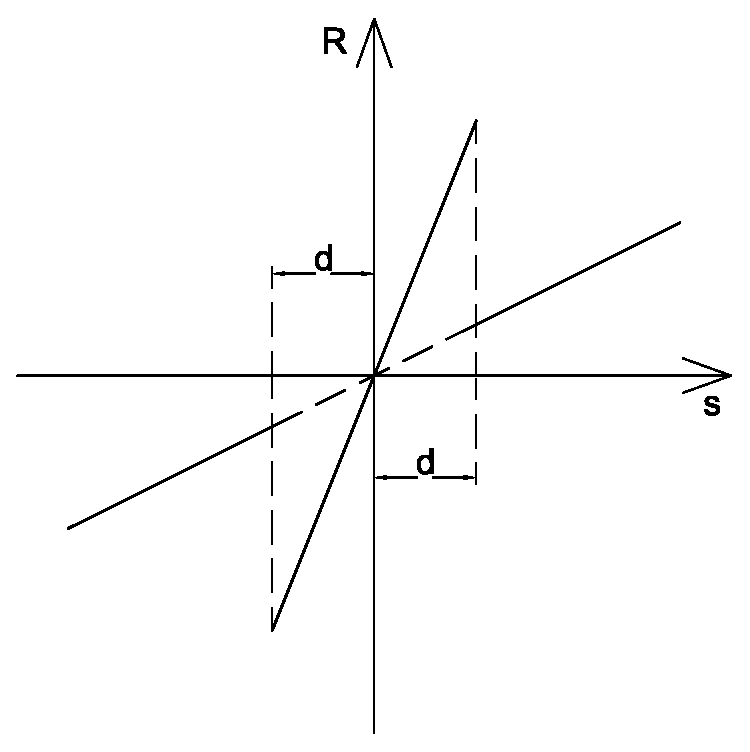
\includegraphics[width=0.4\textwidth]{img/discont.eps}
\caption{Friction characteristics}
\label{fig:fric}
\end{figure}

\subsection{Simulation results}
Despite the fact that the motion planning algorithm based on the endogenous 
configuration approach does not converge in general for discontinuous models,
it came out to be possible to find a set of the parameters for which the algorithm
coupled with the event mechanism produced
a valid result. These parameters are shown in detail in section \ref{sec:discont_params_uni}.
The results --- the error, path, slips and control inputs plots --- are depicted
in figure \ref{fig:pr_uni}.
The behaviour of this motion planning method for discontinuous models has been thoroughly examined,
and the conclusion is that the case presented here is rather special. Mostly, the error rises to the infinity
or oscillates around a certain value.

\begin{figure}
\begin{subfigure}[b]{0.45\textwidth}
\centering
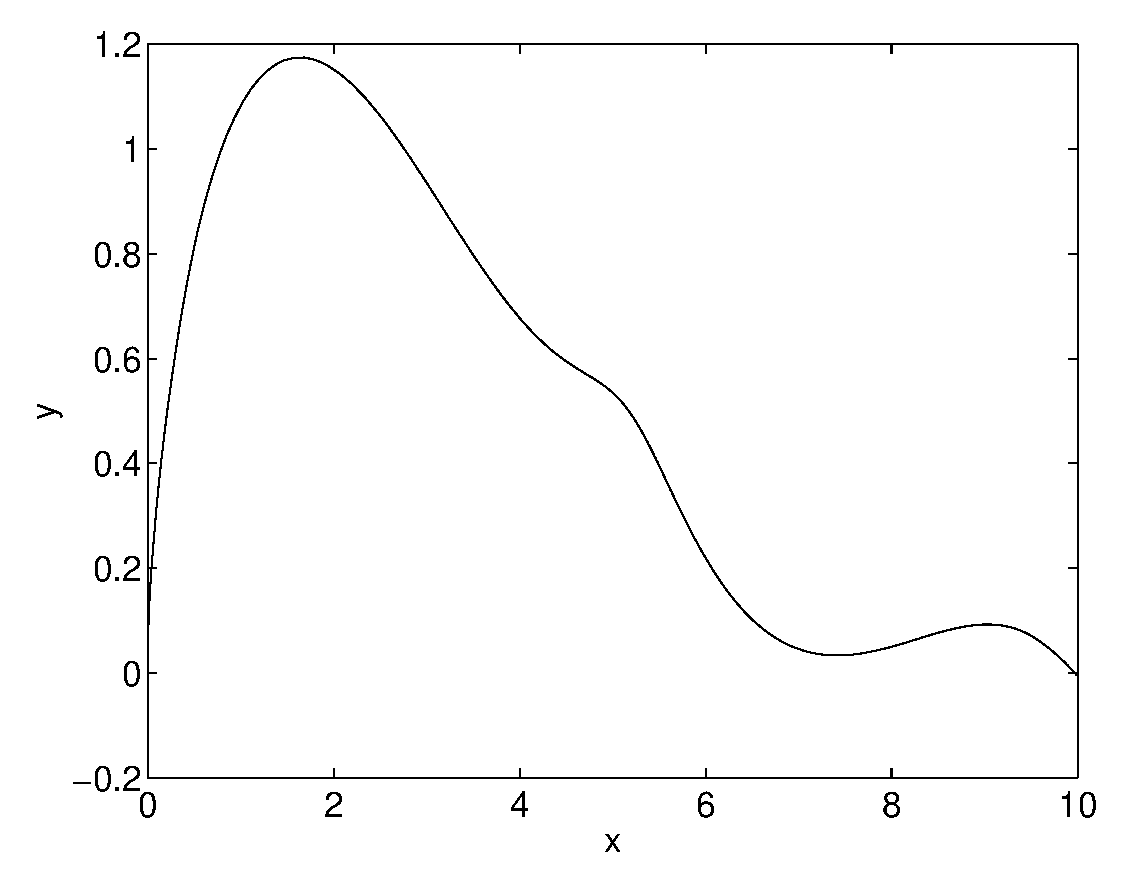
\includegraphics[width=\textwidth]{img/unicycle_path.eps}
\caption{path}
\end{subfigure}
~
\begin{subfigure}[b]{0.45\textwidth}
\centering
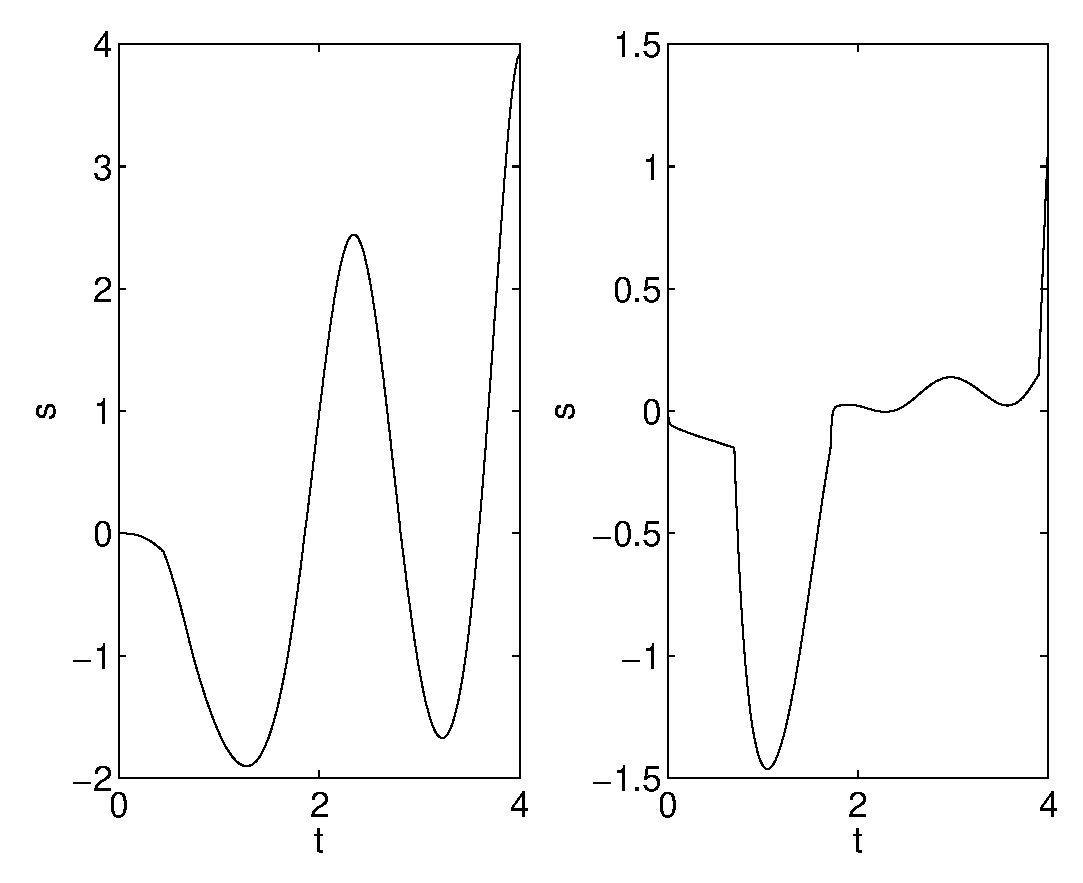
\includegraphics[width=\textwidth]{img/unicycle_slips.eps}
\caption{slips}
\end{subfigure}

\begin{subfigure}[b]{0.45\textwidth}
\centering
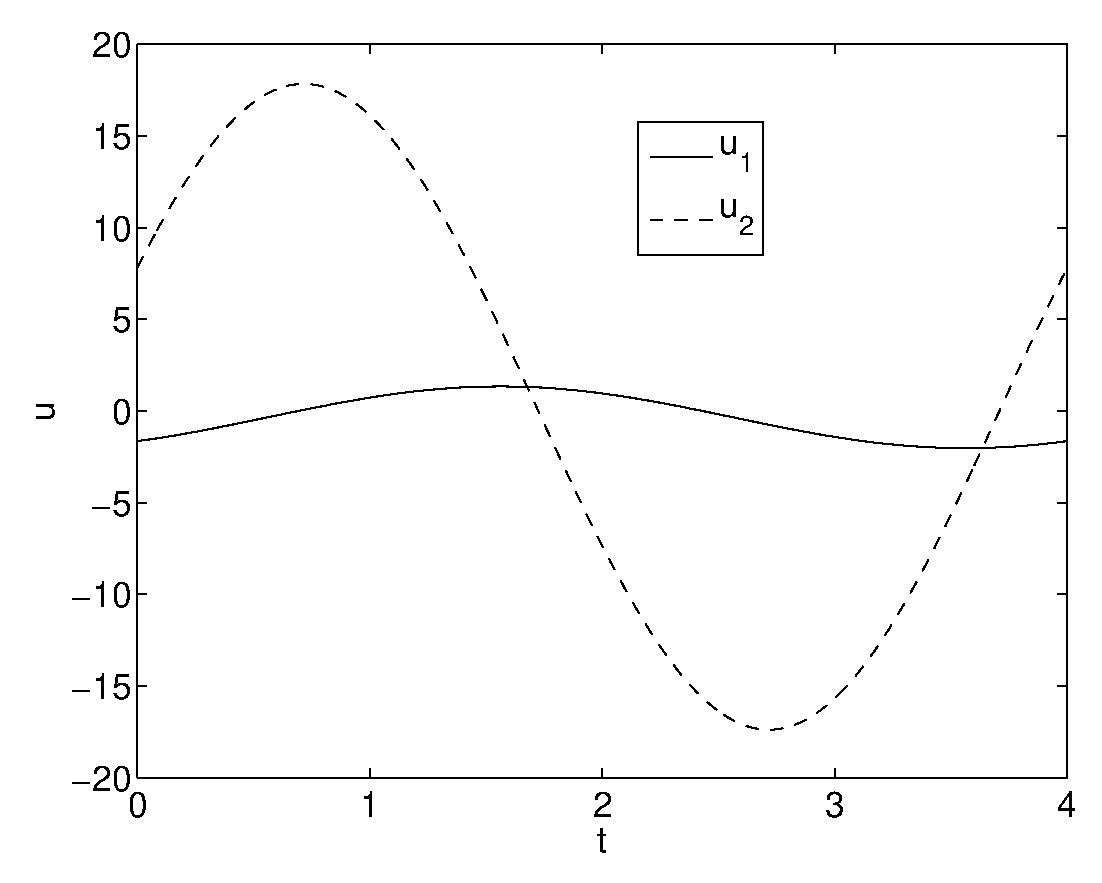
\includegraphics[width=\textwidth]{img/unicycle_u.eps}
\caption{control inputs}
\end{subfigure}
~
\begin{subfigure}[b]{0.45\textwidth}
\centering
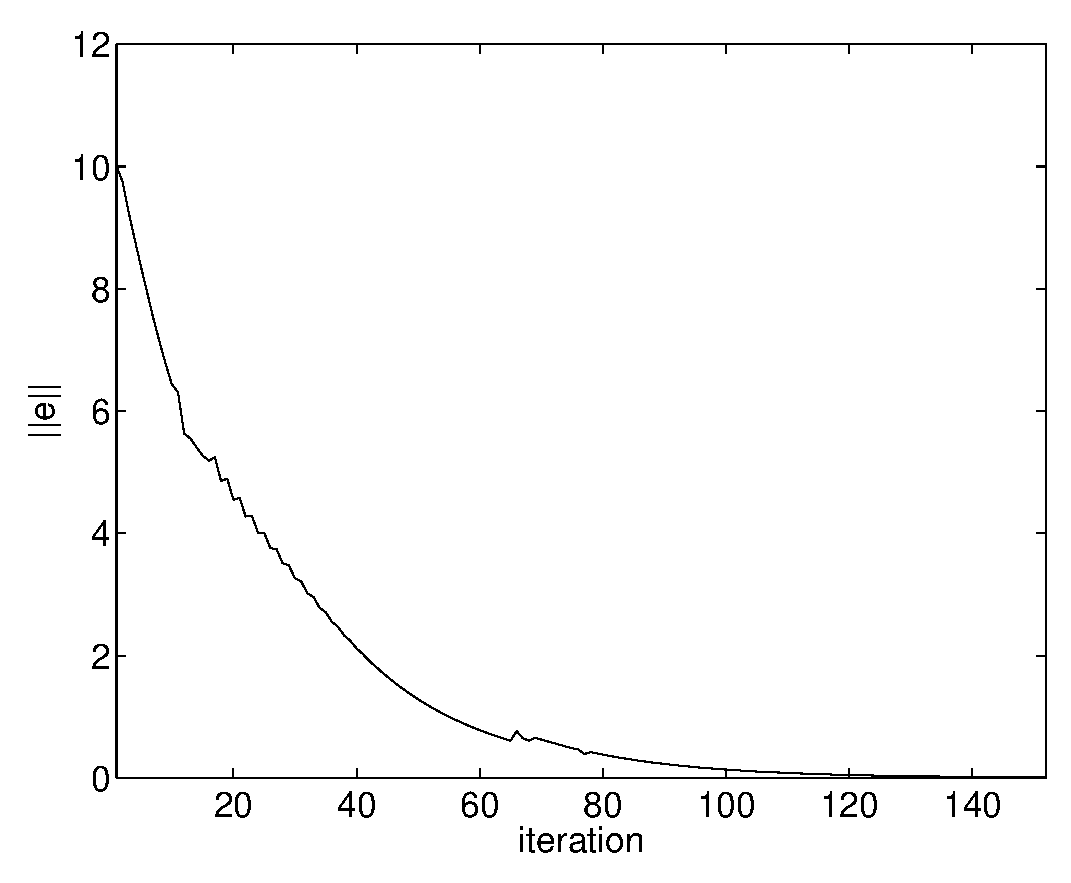
\includegraphics[width=\textwidth]{img/unicycle_err.eps}
\caption{error norm}
\end{subfigure}
\caption{Unicycle, discontinuous friction model}
\label{fig:pr_uni}
\end{figure}

\section{Mobile platform}
\subsection{Problem formulation}
\label{sec:rex_task}
The problem to be solved is to move the platform from the initial state
$q_0 = (w_0, \dot{w}_0)^T = (0, 0, a\frac{\pi}{2}, 0_7)^T$ to the state satisfying the desired
output function value
$y_d=(x_p, y_p, \phi, \dot w)^T = (10, 0, a\frac{\pi}{2}, 0_7)^T$, 
within the given time $T$. 
This corresponds to a parking manoeuvre.
%
%Now two types of friction models will be discussed --- linear
%and discontinuous. These models will be employed in simulations
%regarding solving the above problem.

\subsection{Simulation conditions}
\label{sec:pltf_params}
The platform parameters were set according to \cite{coupled}, and are as follows:
\begin{multicols}{2}
\begin{itemize}
\item $m_p = 21.107\,\mathrm{kg}$,
\item $m_w = 2.380\,\mathrm{kg}$,
\item $a_{p1} = 0.377\,\mathrm{m}$,
\item $a_{p2} = 0.008\,\mathrm{m}$,
\item $a = 0.730\,\mathrm{m}$,
\item $b = 0.350\,\mathrm{m}$,
\item $R = 0.127\,\mathrm{m}$,
\item $I_{p33} = 1.991\,\mathrm{kgm^2}$,
\item $I_{w11} = 0.015\,\mathrm{kgm^2}$,
\item $I_{w33} = 0.009\,\mathrm{kgm^2}$.
\end{itemize}
\end{multicols}
\hspace{-\parindent}Initial conditions for the $\lambda$ parameters used to compute control functions
in \eqref{eq:endogen_num} are
\begin{equation}
\lambda_0=
(\underbrace{0, \ 0.5, \ 0, \ 0, \ 0, \ 0, \ 0,}_{u_1}\ \underbrace{0, \ 0.5, \ 0, \ 0, \ 0, \ 0, \ 0}_{u_2})^T.
\end{equation}
 	

\subsection{Linear friction model}
This model assumes that coefficients $\epsilon_i$ and $\tau_i$ in \eqref{eq:force_r} are constant. Four cases of friction coefficients values have been analysed:
\begin{enumerate}
\item $\epsilon_i=15$ and $\tau_i=15$,
\item $\epsilon_i=15$ and $\tau_i=1$,
\item $\epsilon_i=1$ and $\tau_i=15$,
\item $\epsilon_i=1$ and $\tau_i=1$,
\end{enumerate}
for $i=1,\,2,\,3,\,4$.
Every case was studied on two different control time horizons 10\,s and 20\,s. The results of the
simulations are shown in figures \ref{fig:pl1}--\ref{fig:pl8}.

It is also worth to check, whether the input functions obtained in simulations
are feasible on the real object. The total energy of the signal was computed as $\int_0^T u^2\ud t$
and the maximal amplitude which can be compared to the maximum torque achievable by the real actuator.
These values, computed for all the simulations run, are presented in table \ref{tab:control}.
\begin{table}[h]
\centering
\caption{Control input parameters, continuous platform model}
\label{tab:control}
\begin{tabular}{rrr|r|r|r|r|}
\cline{4-7}
\multicolumn{1}{c}{}                      & \multicolumn{1}{c}{}                     & \multicolumn{1}{c|}{}            & \multicolumn{2}{c|}{energy: $\int_0^Tu_i^2(t)\ud t$}                             & \multicolumn{2}{c|}{amplitude [Nm]}                          \\ \hline
\multicolumn{1}{|c|}{$\tau$}              & \multicolumn{1}{c|}{$\epsilon$}          & \multicolumn{1}{c|}{$T$ {[}s{]}} & \multicolumn{1}{c|}{$u_1$} & \multicolumn{1}{c|}{$u_2$} & \multicolumn{1}{c|}{$u_1$} & \multicolumn{1}{c|}{$u_2$} \\ \hline
\multicolumn{1}{|r|}{\multirow{4}{*}{1}}  & \multicolumn{1}{r|}{\multirow{2}{*}{1}}  & 20                               & 5906                       & 805                        & 3.16                       & 1.26                       \\ \cline{3-7} 
\multicolumn{1}{|r|}{}                    & \multicolumn{1}{r|}{}                    & 10                               & 19337                      & 2036                       & 8.03                       & 3.09                       \\ \cline{2-7} 
\multicolumn{1}{|r|}{}                    & \multicolumn{1}{r|}{\multirow{2}{*}{15}} & 20                               & 118900                     & 21301                      & 14.07                      & 6.03                       \\ \cline{3-7} 
\multicolumn{1}{|r|}{}                    & \multicolumn{1}{r|}{}                    & 10                               & 662430                     & 309980                     & 48.38                      & 31.56                      \\ \hline
\multicolumn{1}{|r|}{\multirow{4}{*}{15}} & \multicolumn{1}{r|}{\multirow{2}{*}{1}}  & 20                               & 5906                       & 805                        & 3.16                       & 1.26                       \\ \cline{3-7} 
\multicolumn{1}{|r|}{}                    & \multicolumn{1}{r|}{}                    & 10                               & 19335                      & 2034                       & 8.03                       & 3.09                       \\ \cline{2-7} 
\multicolumn{1}{|r|}{}                    & \multicolumn{1}{r|}{\multirow{2}{*}{15}} & 20                               & 118900                     & 21298                      & 14.06                      & 6.00                       \\ \cline{3-7} 
\multicolumn{1}{|r|}{}                    & \multicolumn{1}{r|}{}                    & 10                               & 661100                     & 309080                     & 48.36                      & 31.56                      \\ \hline
\end{tabular}
\end{table}
\begin{figure}[h]
\begin{subfigure}[b]{\textwidth}
\centering
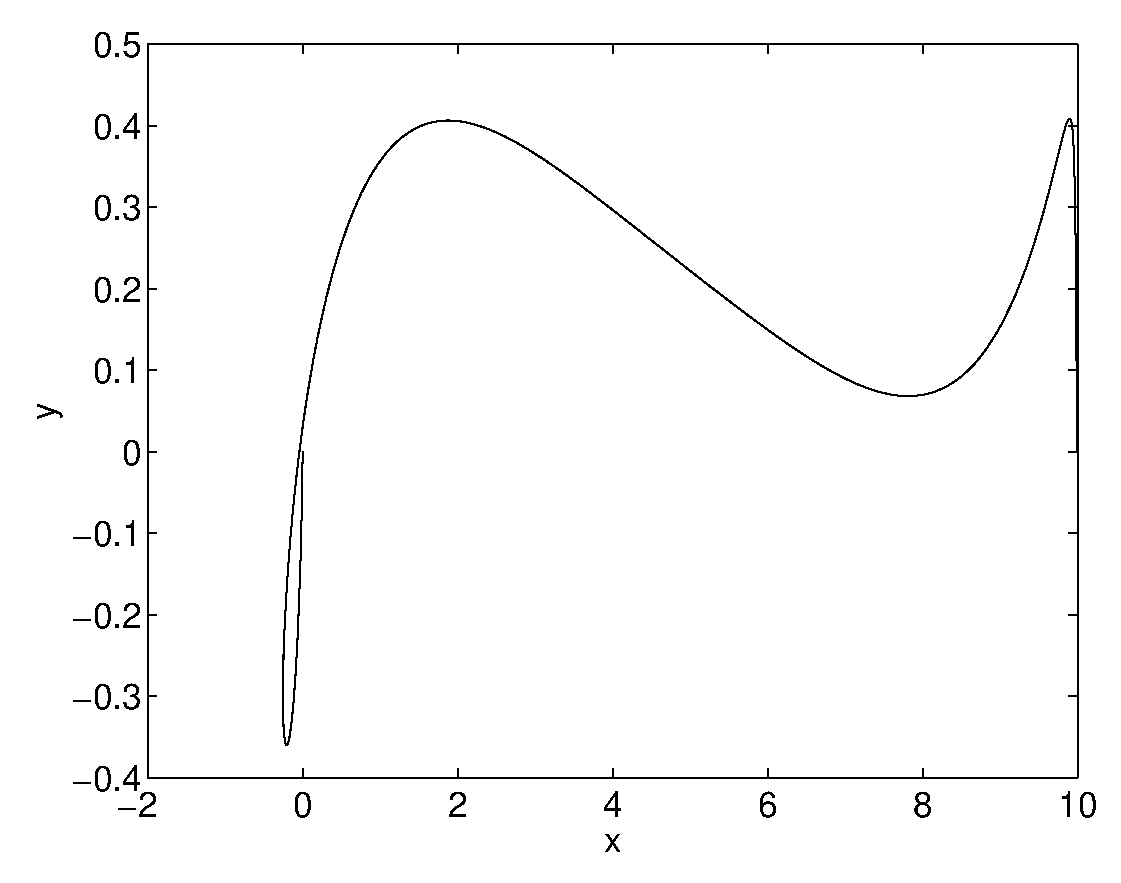
\includegraphics[height=0.3\textheight]{img/final_15_1_10_path.eps}
\caption{path}
\end{subfigure}

\begin{subfigure}[b]{\textwidth}
\centering
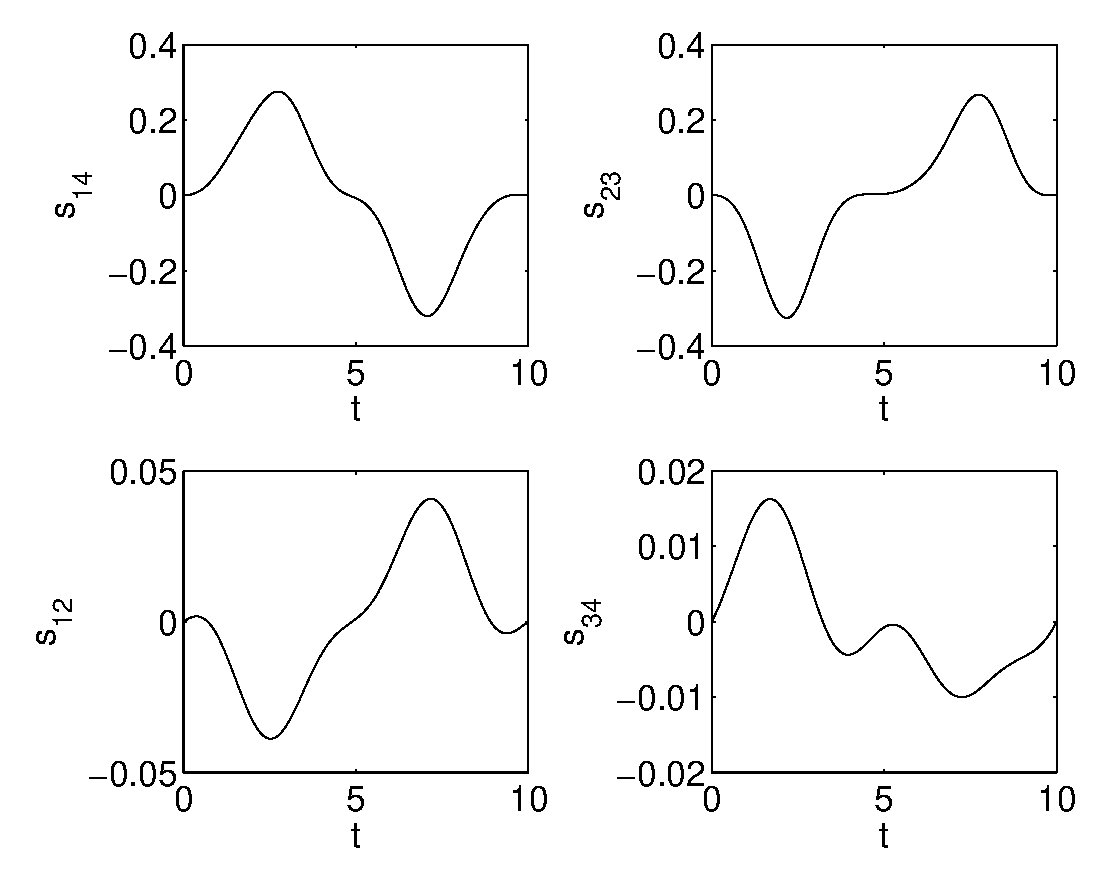
\includegraphics[height=0.3\textheight]{img/final_15_1_10_slips.eps}
\caption{slips}
\end{subfigure}

\begin{subfigure}[b]{\textwidth}
\centering
\includegraphics[height=0.3\textheight]{img/final_15_1_10_u.eps}
\caption{path}
\end{subfigure}
\caption{whole sim $T=10$}
\end{figure}

\begin{figure}[h]
\begin{subfigure}[b]{\textwidth}
\centering
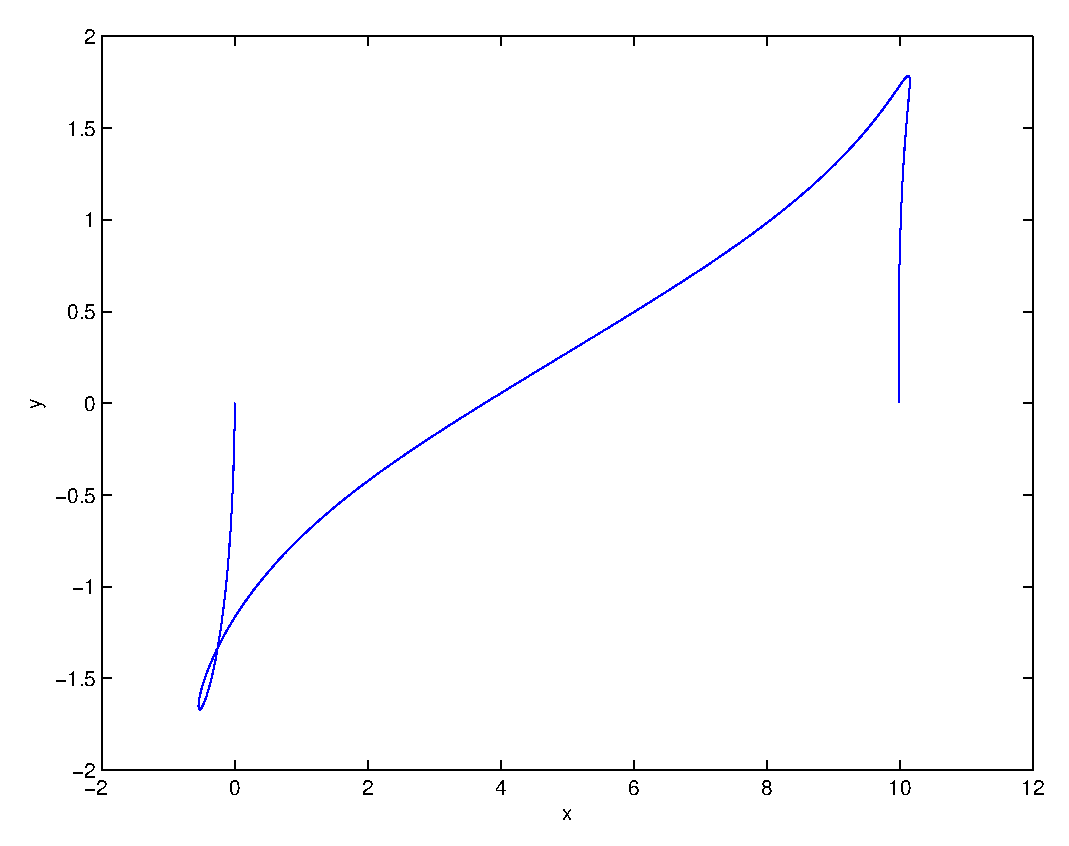
\includegraphics[height=0.3\textheight]{img/final_15_1_20_path.eps}
\caption{path}
\end{subfigure}

\begin{subfigure}[b]{\textwidth}
\centering
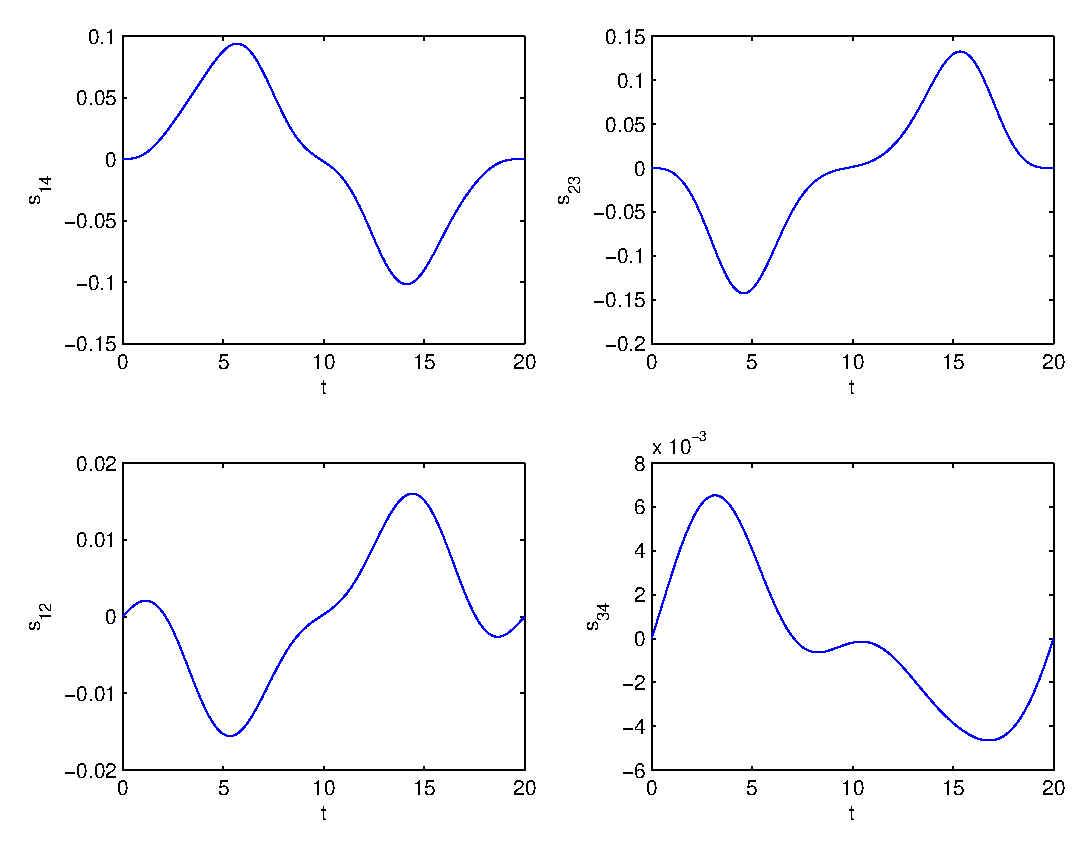
\includegraphics[height=0.3\textheight]{img/final_15_1_20_slips.eps}
\caption{slips}
\end{subfigure}

\begin{subfigure}[b]{\textwidth}
\centering
\includegraphics[height=0.3\textheight]{img/final_15_1_20_u.eps}
\caption{path}
\end{subfigure}
\caption{whole sim $T=20$}
\end{figure}

%%%%%%%%%%%%%%%%%%%%%%%%%%%%%%%%%%%%%%%%%%%%%%%%%%%%%%%%%%%%%%%%%%%%%%%%%%%%%%%%%%%%%%%%%%%
%%%%%%%%%%%%%%%%%%%%%%%%%%%%%%%%%%%%%%%%%%%%%%%%%%%%%%%%%%%%%%%%%%%%%%%%%%%%%%%%%%%%%%%%%%%
%%%%%%%%%%%%%%%%%%%%%%%%%%%%%%%%%%%%%%%%%%%%%%%%%%%%%%%%%%%%%%%%%%%%%%%%%%%%%%%%%%%%%%%%%%%
%%%%%%%%%%%%%%%%%%%%%%%%%%%%%%%%%%%%%%%%%%%%%%%%%%%%%%%%%%%%%%%%%%%%%%%%%%%%%%%%%%%%%%%%%%%
%%%%%%%%%%%%%%%%%%%%%%%%%%%%%%%%%%%%%%%%%%%%%%%%%%%%%%%%%%%%%%%%%%%%%%%%%%%%%%%%%%%%%%%%%%%

\begin{figure}[h]
\begin{subfigure}[b]{\textwidth}
\centering
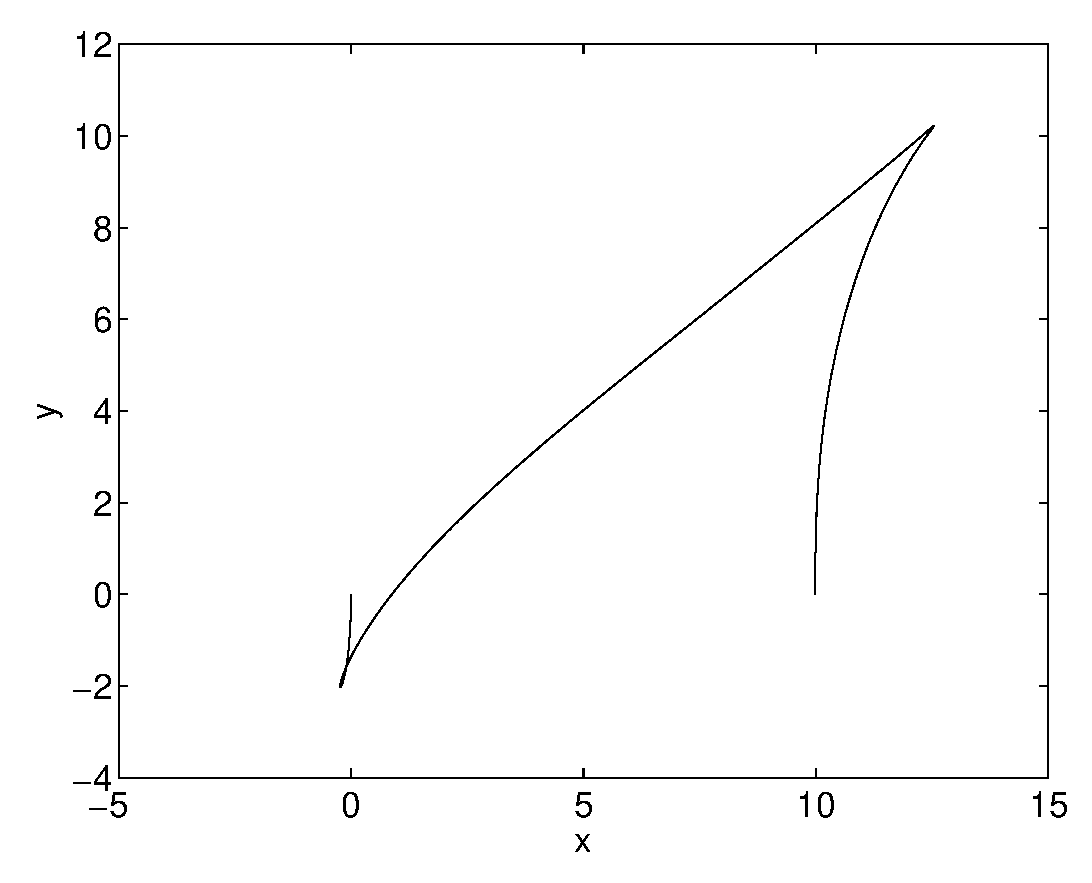
\includegraphics[height=0.3\textheight]{img/final_15_15_10_path.eps}
\caption{path}
\end{subfigure}

\begin{subfigure}[b]{\textwidth}
\centering
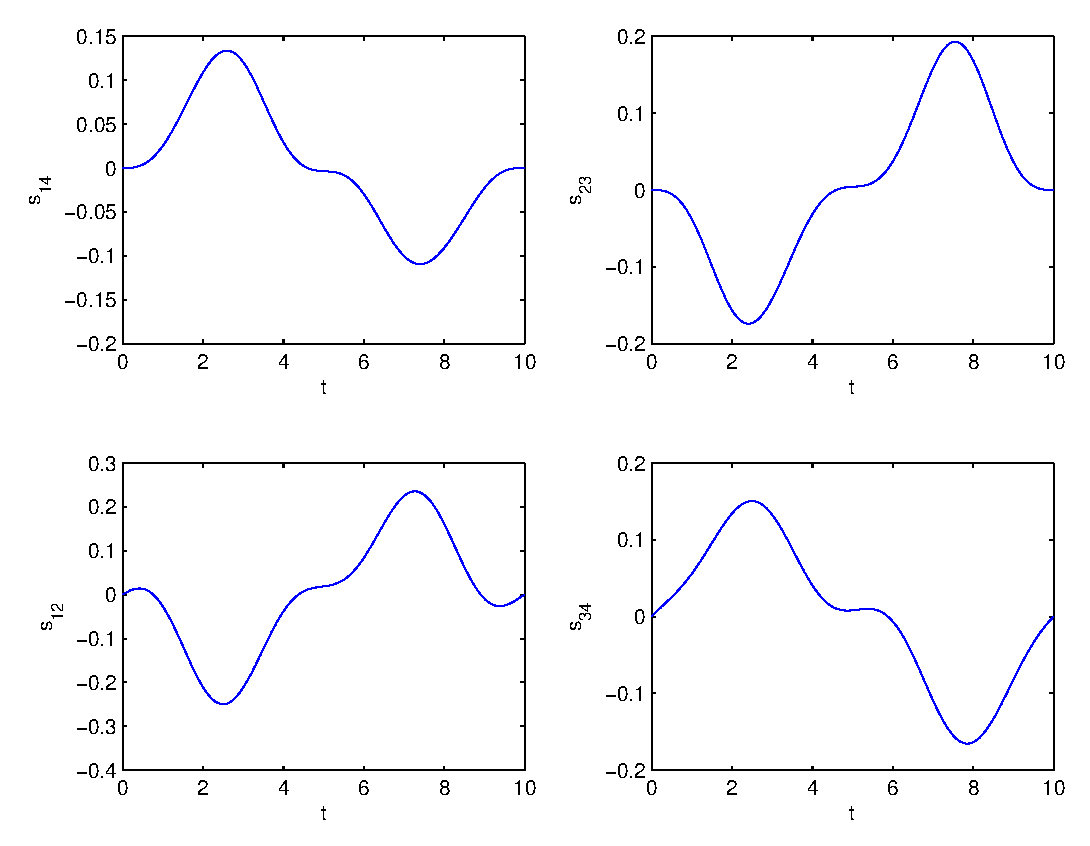
\includegraphics[height=0.3\textheight]{img/final_15_15_10_slips.eps}
\caption{slips}
\end{subfigure}

\begin{subfigure}[b]{\textwidth}
\centering
\includegraphics[height=0.3\textheight]{img/final_15_15_10_u.eps}
\caption{path}
\end{subfigure}
\caption{whole sim $T=10$}
\end{figure}

\begin{figure}[h]
\begin{subfigure}[b]{\textwidth}
\centering
\includegraphics[height=0.3\textheight]{img/final_15_15_20_path.eps}
\caption{path}
\end{subfigure}

\begin{subfigure}[b]{\textwidth}
\centering
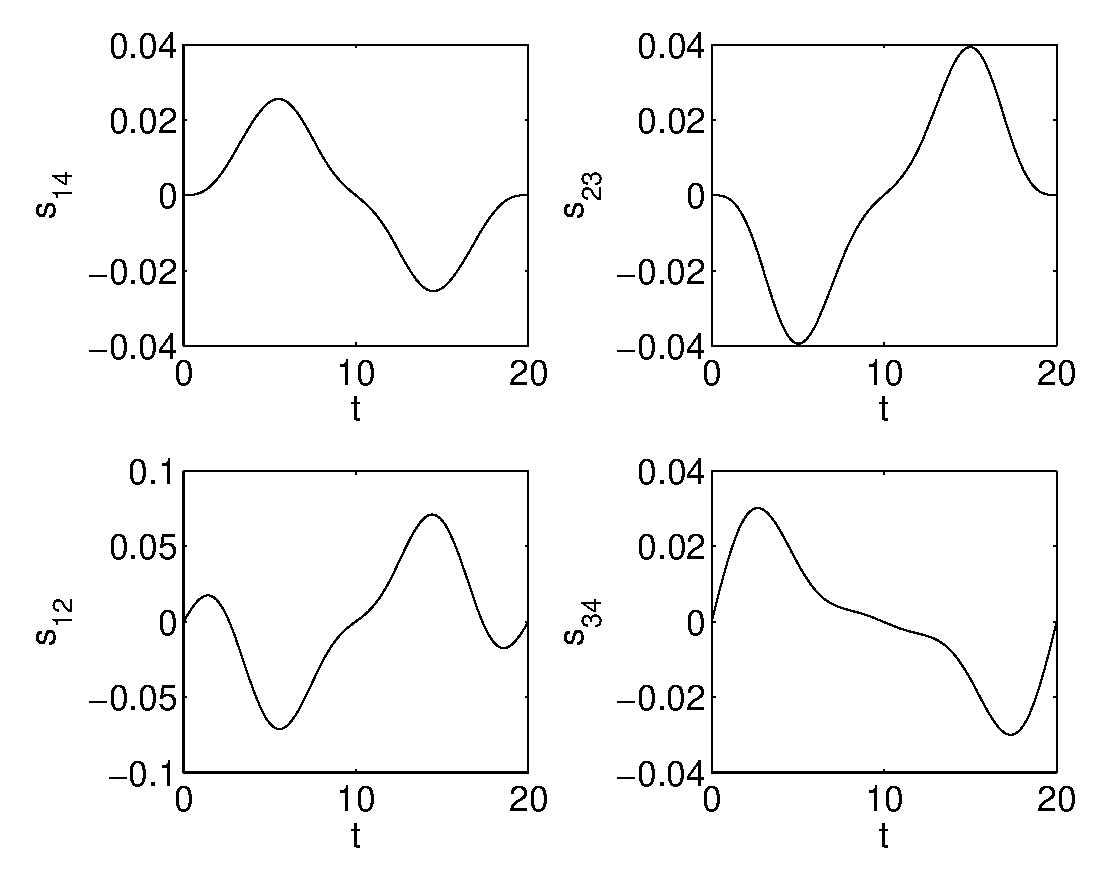
\includegraphics[height=0.3\textheight]{img/final_15_15_20_slips.eps}
\caption{slips}
\end{subfigure}

\begin{subfigure}[b]{\textwidth}
\centering
\includegraphics[height=0.3\textheight]{img/final_15_15_20_u.eps}
\caption{path}
\end{subfigure}
\caption{whole sim $T=20$}
\end{figure}

%%%%%%%%%%%%%%%%%%%%%%%%%%%%%%%%%%%%%%%%%%%%%%%%%%%%%%%%%%%%%%%%%%%%%%%%%%%%%%%%%%%%%%%%%%%
%%%%%%%%%%%%%%%%%%%%%%%%%%%%%%%%%%%%%%%%%%%%%%%%%%%%%%%%%%%%%%%%%%%%%%%%%%%%%%%%%%%%%%%%%%%
%%%%%%%%%%%%%%%%%%%%%%%%%%%%%%%%%%%%%%%%%%%%%%%%%%%%%%%%%%%%%%%%%%%%%%%%%%%%%%%%%%%%%%%%%%%
%%%%%%%%%%%%%%%%%%%%%%%%%%%%%%%%%%%%%%%%%%%%%%%%%%%%%%%%%%%%%%%%%%%%%%%%%%%%%%%%%%%%%%%%%%%
%%%%%%%%%%%%%%%%%%%%%%%%%%%%%%%%%%%%%%%%%%%%%%%%%%%%%%%%%%%%%%%%%%%%%%%%%%%%%%%%%%%%%%%%%%%
\begin{figure}[h]
\begin{subfigure}[b]{\textwidth}
\centering
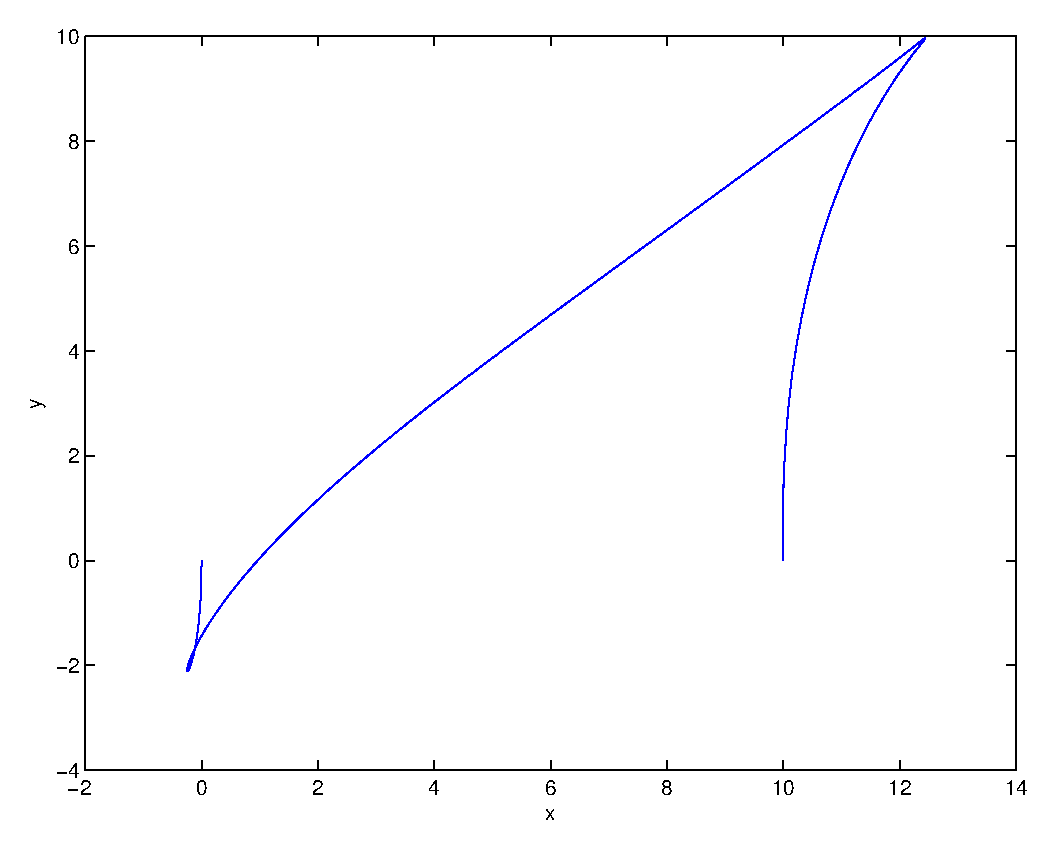
\includegraphics[height=0.3\textheight]{img/final_1_15_10_path.eps}
\caption{path}
\end{subfigure}

\begin{subfigure}[b]{\textwidth}
\centering
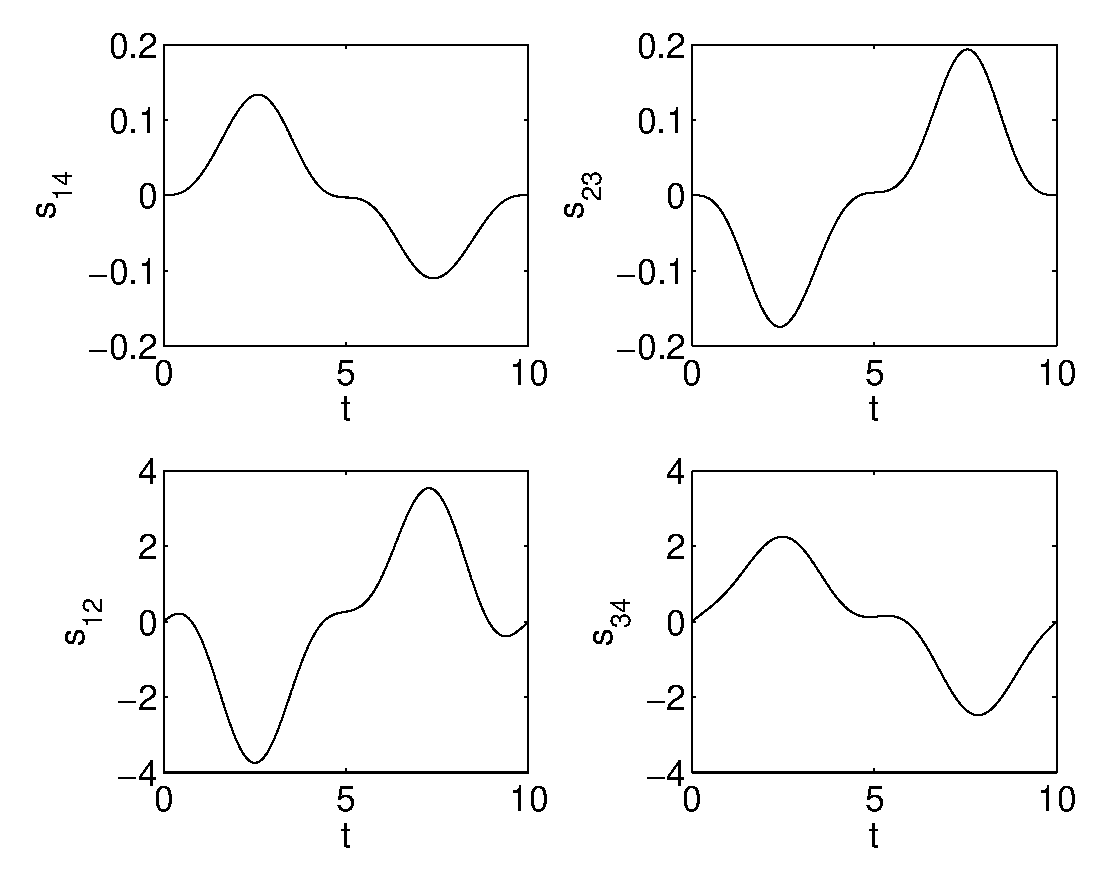
\includegraphics[height=0.3\textheight]{img/final_1_15_10_slips.eps}
\caption{slips}
\end{subfigure}

\begin{subfigure}[b]{\textwidth}
\centering
\includegraphics[height=0.3\textheight]{img/final_1_15_10_u.eps}
\caption{path}
\end{subfigure}
\caption{whole sim $T=10$}
\end{figure}

\begin{figure}[h]
\begin{subfigure}[b]{\textwidth}
\centering
\includegraphics[height=0.3\textheight]{img/final_1_15_20_path.eps}
\caption{path}
\end{subfigure}

\begin{subfigure}[b]{\textwidth}
\centering
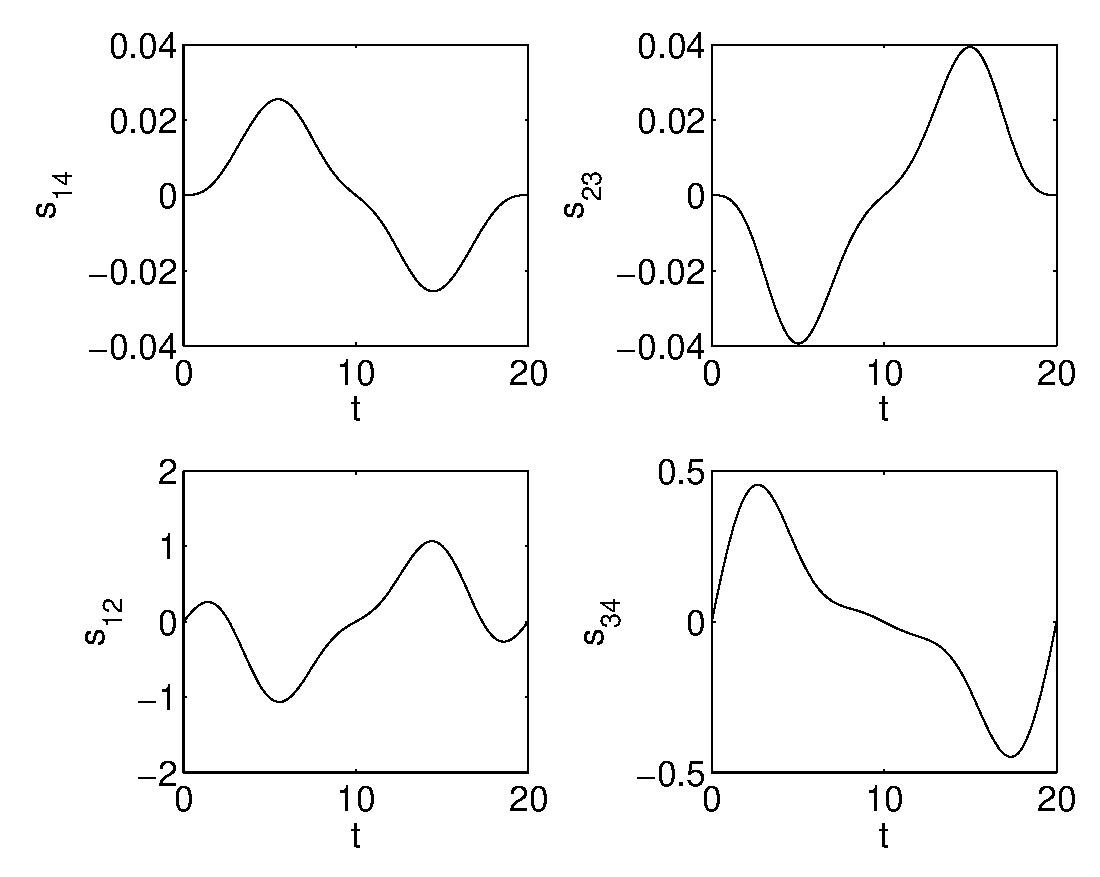
\includegraphics[height=0.3\textheight]{img/final_1_15_20_slips.eps}
\caption{slips}
\end{subfigure}

\begin{subfigure}[b]{\textwidth}
\centering
\includegraphics[height=0.3\textheight]{img/final_1_15_20_u.eps}
\caption{path}
\end{subfigure}
\caption{whole sim $T=20$}
\end{figure}

%%%%%%%%%%%%%%%%%%%%%%%%%%%%%%%%%%%%%%%%%%%%%%%%%%%%%%%%%%%%%%%%%%%%%%%%%%%%%%%%%%%%%%%%%%%
%%%%%%%%%%%%%%%%%%%%%%%%%%%%%%%%%%%%%%%%%%%%%%%%%%%%%%%%%%%%%%%%%%%%%%%%%%%%%%%%%%%%%%%%%%%
%%%%%%%%%%%%%%%%%%%%%%%%%%%%%%%%%%%%%%%%%%%%%%%%%%%%%%%%%%%%%%%%%%%%%%%%%%%%%%%%%%%%%%%%%%%
%%%%%%%%%%%%%%%%%%%%%%%%%%%%%%%%%%%%%%%%%%%%%%%%%%%%%%%%%%%%%%%%%%%%%%%%%%%%%%%%%%%%%%%%%%%
%%%%%%%%%%%%%%%%%%%%%%%%%%%%%%%%%%%%%%%%%%%%%%%%%%%%%%%%%%%%%%%%%%%%%%%%%%%%%%%%%%%%%%%%%%%
\begin{figure}[h]
\begin{subfigure}[b]{\textwidth}
\centering
\includegraphics[height=0.3\textheight]{img/final_1_1_10_path.eps}
\caption{path}
\end{subfigure}

\begin{subfigure}[b]{\textwidth}
\centering
\includegraphics[height=0.3\textheight]{img/final_1_1_10_slips.eps}
\caption{slips}
\end{subfigure}

\begin{subfigure}[b]{\textwidth}
\centering
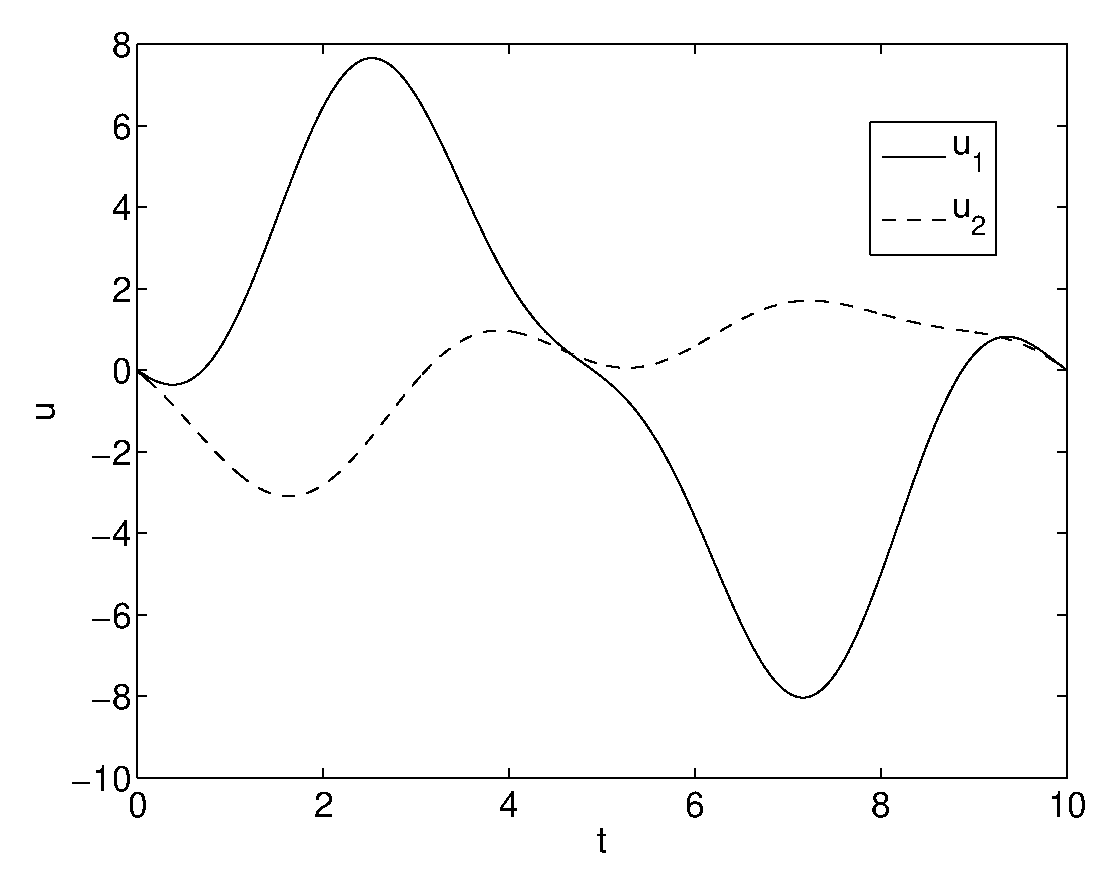
\includegraphics[height=0.3\textheight]{img/final_1_1_10_u.eps}
\caption{path}
\end{subfigure}
\caption{whole sim $T=10$}
\end{figure}

\begin{figure}[h]
\begin{subfigure}[b]{\textwidth}
\centering
\includegraphics[height=0.3\textheight]{img/final_1_1_20_path.eps}
\caption{path}
\end{subfigure}

\begin{subfigure}[b]{\textwidth}
\centering
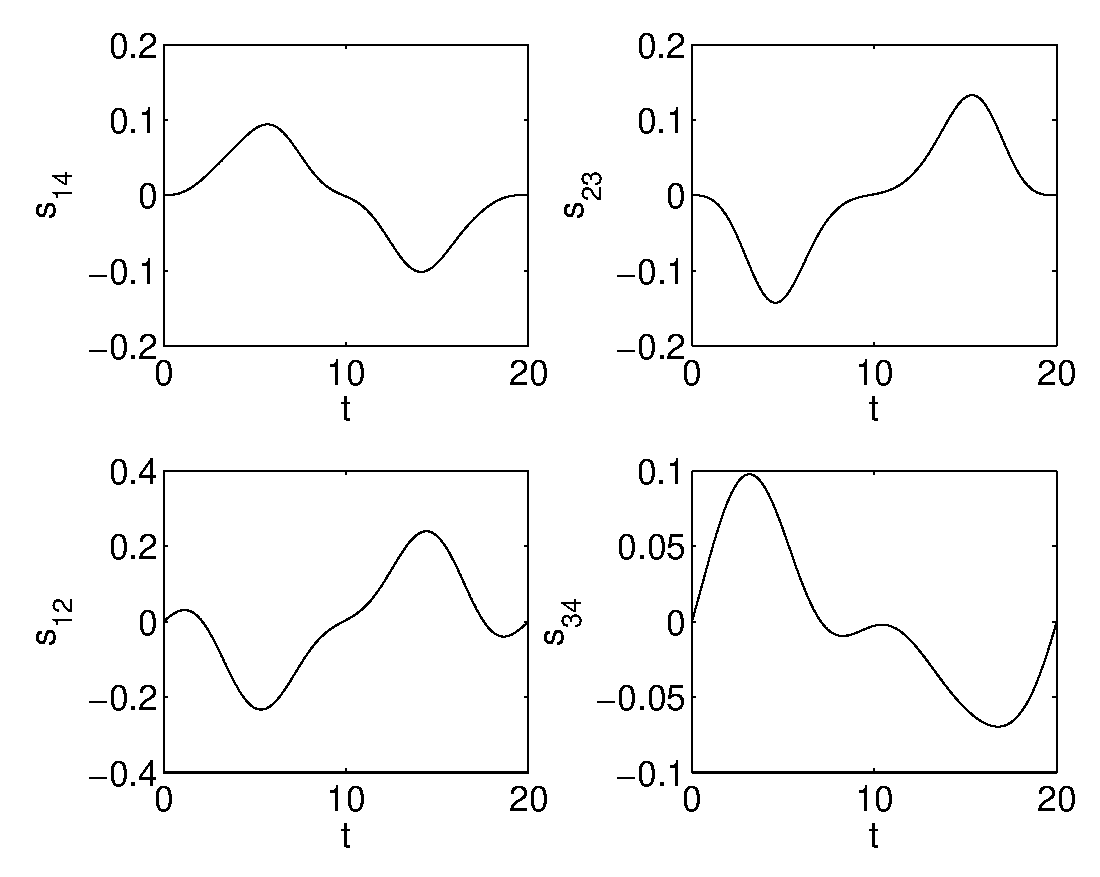
\includegraphics[height=0.3\textheight]{img/final_1_1_20_slips.eps}
\caption{slips}
\end{subfigure}

\begin{subfigure}[b]{\textwidth}
\centering
\includegraphics[height=0.3\textheight]{img/final_1_1_20_u.eps}
\caption{path}
\end{subfigure}
\caption{whole sim $T=20$}
\end{figure}

%%%%%%%%%%%%%%%%%%%%%%%%%%%%%%%%%%%%%%%%%%%%%%%%%%%%%%%%%%%%%%%%%%%%%%%%%%%%%%%%%%%%%%%%%%%
%%%%%%%%%%%%%%%%%%%%%%%%%%%%%%%%%%%%%%%%%%%%%%%%%%%%%%%%%%%%%%%%%%%%%%%%%%%%%%%%%%%%%%%%%%%
%%%%%%%%%%%%%%%%%%%%%%%%%%%%%%%%%%%%%%%%%%%%%%%%%%%%%%%%%%%%%%%%%%%%%%%%%%%%%%%%%%%%%%%%%%%
%%%%%%%%%%%%%%%%%%%%%%%%%%%%%%%%%%%%%%%%%%%%%%%%%%%%%%%%%%%%%%%%%%%%%%%%%%%%%%%%%%%%%%%%%%%
%%%%%%%%%%%%%%%%%%%%%%%%%%%%%%%%%%%%%%%%%%%%%%%%%%%%%%%%%%%%%%%%%%%%%%%%%%%%%%%%%%%%%%%%%%%

\subsection{Discontinuous friction model}
In this model coefficients $\epsilon_i$ and $\tau_i$ in \eqref{eq:force_r} depend
on the value of the slip. The idea of such a friction model has been described
in section \ref{sec:discont_params_uni}. With such an approach the formulae defining
friction coefficients are of the form
\begin{equation*}
\begin{aligned}
\epsilon_1=\epsilon_4&=\begin{cases}
\epsilon_{high} &\mbox{if } |s_{14}| \leq d \\
\epsilon_{low} &\mbox{if } |s_{14}| > d
\end{cases}, &
\tau_1=\tau_2&=\begin{cases}
\tau_{high} &\mbox{if } |s_{12}| \leq d \\
\tau_{low} &\mbox{if } |s_{12}| > d
\end{cases},\\
\epsilon_2=\epsilon_3&=\begin{cases}
\epsilon_{high} &\mbox{if } |s_{23}| \leq d \\
\epsilon_{low} &\mbox{if } |s_{23}| > d
\end{cases}, &
\tau_3=\tau_4&=\begin{cases}
\tau_{high} &\mbox{if } |s_{34}| \leq d \\
\tau_{low} &\mbox{if } |s_{34}| > d
\end{cases}.
\end{aligned}
\end{equation*}
Two sets of friction parameters has been used in the simulations:
\begin{enumerate}
\item $\epsilon_{high}=5$, $\epsilon_{low}=0.05$,
$\tau_{high}=5$, $\tau_{low}=0.05$, $d=0.2$;
\item $\epsilon_{high}=5$, $\epsilon_{low}=1$,
$\tau_{high}=5$, $\tau_{low}=1$, $d=0.2$.
\end{enumerate}
Unfortunately, there is no guarantee for the
algorithm to converge for a discontinuous model and such a situation takes place in
the case 1. The plot of the error norm with respect to the iteration number is shown
in figure \ref{fig:error_discont}. It is clearly visible that the plot of the
error norm is not monotonic. The reason why the endogenous configuration approach
does not perform well here is the fundamental idea underlying motion planning algorithm.
It assumes that a small change in endogenous configuration results in a small change
in the output function value. This statement is true for continuous models. On the contrary,
when a model includes some discontinuities, even a small variation to the input may take
the system to a distant point from the original one in the output space. Therefore, the
error may increase in the next iteration of the algorithm. Note that decreasing
the $\gamma$ parameter in equation \eqref{eq:endogen_num} will not solve this problem either.
In other words, if the platform loses the traction in a different point than in
the previous iteration, it ends up in a place not related to the one supposed to be
according to the algorithm, because actually the model has changed in the meanwhile.

A contrasting situation takes place while using the set of parameters No. 2. Due to the fact
that the friction coefficients do not differ too much, the algorithm manages to converge.
In such circumstances switching the friction coefficient does not result in a large change to the model.
Figure \ref{fig:pr_discont_ok} demonstrates the results for this case. The characteristics
of the obtained control inputs are shown in table \ref{tab:in_discont_ok}

\begin{figure}[htp]
\centering
\includegraphics[height=0.3\textheight]{img/discont_err.eps}
\caption{Error norm w.r.t iteration, discontinuous platform model No. 1}
\label{fig:error_discont}
\end{figure}

\begin{table}[htb]
\caption{Control input parameters, discontinuous platform model, problem 2}
\label{tab:in_discont_ok}
\centering
\begin{tabular}{|r|r|r|r|}
\hline
\multicolumn{2}{|c|}{energy: $\int_0^Tu_i^2(t)\ud t$}                             & \multicolumn{2}{c|}{amplitude [$\mathrm{Nm}$]}                          \\ \hline
\multicolumn{1}{|c|}{$u_1$} & \multicolumn{1}{c|}{$u_2$} & \multicolumn{1}{c|}{$u_1$} & \multicolumn{1}{c|}{$u_2$} \\ \hline
1101                       & 230                        & 23.88                      & 14.16                      \\ \hline
\end{tabular}
\end{table}

\begin{figure}[h]
\begin{subfigure}[b]{0.45\textwidth}
\centering
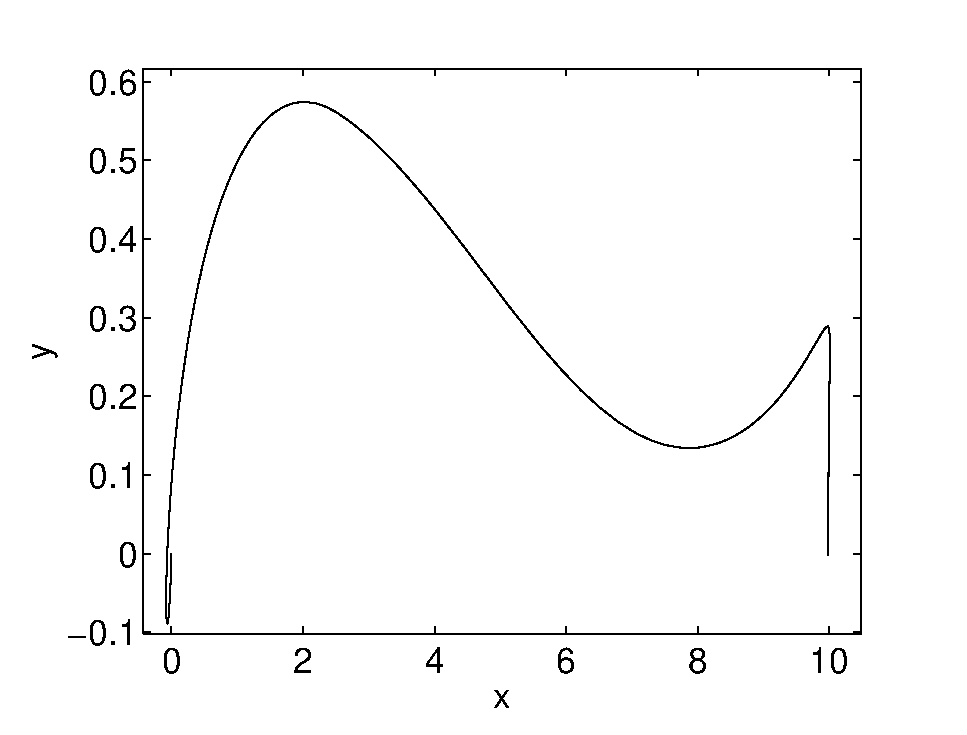
\includegraphics[width=\textwidth]{img/discont_ok_path.eps}
\caption{path}
\end{subfigure}
~
\begin{subfigure}[b]{0.45\textwidth}
\centering
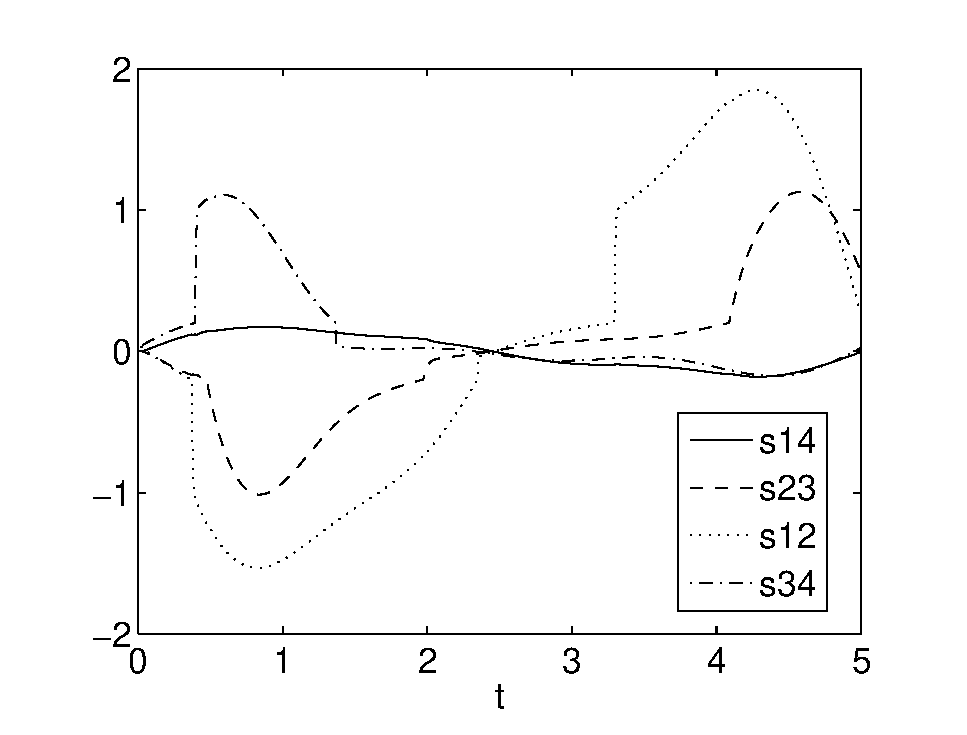
\includegraphics[width=\textwidth]{img/discont_ok_slips.eps}
\caption{slips}
\end{subfigure}

\begin{subfigure}[b]{0.45\textwidth}
\centering
\includegraphics[width=\textwidth]{img/discont_ok_u.eps}
\caption{control inputs}
\end{subfigure}
~
\begin{subfigure}[b]{0.45\textwidth}
\centering
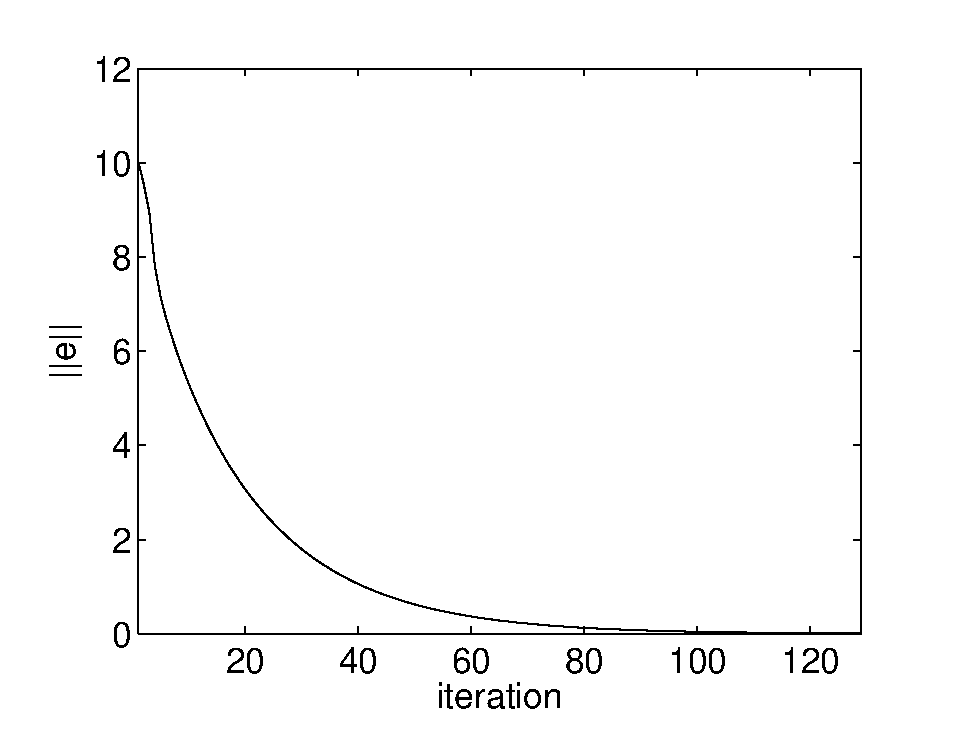
\includegraphics[width=\textwidth]{img/discont_ok_err.eps}
\caption{error norm}
\end{subfigure}
\caption{Mobile platform, second discontinuous friction model}
\label{fig:pr_discont_ok}
\end{figure}

\section{Mobile manipulator}
This section covers the simulations of the whole RobRex mobile manipulator. Two types of problems will
be discussed here: output function regarding only the end-effector task space coordinates
and output function containing both mobile platform and effector coordinates.
\subsection{Problem formulation}
The initial conditions for both tasks are: $q_0 = (w_0, \dot{w}_0)^T = (0, 0, a\frac{\pi}{2}, 0_7)^T$, 
$x_0 = \left(
x_1 ,\, x_2 ,\, x_4 ,\, x_5
\right) = \left(
\frac{\pi}{4} ,\, \frac{\pi}{5} ,\, \frac{\pi}{6} ,\, -\frac{\pi}{3}
\right).$ The control horizon for these tasks is $T=20\,\mathrm{s}$.
\subsubsection{Problem 1}
This motion planning problem regards only the final position of the effector
and the velocities of the platform. 
The following output function value $k(q, x) = (x_e, y_e, z_e, \phi, \theta, \psi, \dot w) $ should be equal to
$(10, 0, 0.2, \frac{\pi}{2}, \frac{\pi}{4}, -\frac{\pi}{2}, 0_5)$, where
$x_e$, $y_e$, $z_e$ are the task space coordinates and $\phi$, $\theta$, $\psi$
are Euler angles of the effector (see section \ref{sec:manipul}). The zero-velocity
requirements guarantee that the whole system will stand still at the end
of the motion.
\subsubsection{Problem 2}
This case is related to the platform pose as well as to the configuration of the effector.
As far as the platform is concerned, the constraints are imposed only on the $x_p$ coordinate and
the velocities. Let us define the output function as $k(q, x) = (x_p, \dot w, y_e, \phi, \theta, \psi)$.
As for the platform, the desired values are
$(x_p, \dot{w}) = (10, 0, 0, 0, 0, 0)$. When it comes to
the effector, we want to reach the following point in the task space: $(y_e, \phi, \theta, \psi)
= (0, \frac{\pi}{2}, \frac{\pi}{4}, -\frac{\pi}{2})$.

\subsection{Simulation conditions}
The platform parameters has been set as in section \ref{sec:pltf_params}. The lenghts of the links
are as follows: $a_1=0 \,\mathrm{m}$,
$a_2=0.1276 \,\mathrm{m}$,
$a_3=0.041 \,\mathrm{m}$,
$a_4=0.2615 \,\mathrm{m}$,
$a_5=0.0195 \,\mathrm{m}$.

\subsection{Simulation results}
The outcomes of the simulations are presented in figure \ref{fig:pr1} for the problem 1 and in figure
\ref{fig:pr2} for the problem 2. These figures include the plots of the error vs. the
iteration, the platform path, the slip values, and the inputs. The joint angles are
presented in table \ref{tab:effector}. Regarding the control parameters, table \ref{tab:in_eff}
shows the total energy of the signal and its maximum amplitude.

\begin{table}[!htb]
\caption{Control parameters, mobile manipulator}
\label{tab:in_eff}
\centering
\begin{tabular}{l|r|r|r|r|}
\cline{2-5}
\multicolumn{1}{c|}{}             & \multicolumn{2}{c|}{energy: $\int_0^Tu_i^2(t)\ud t$}                             & \multicolumn{2}{c|}{amplitude [$\mathrm{Nm}$]}                          \\ \cline{2-5} 
\multicolumn{1}{c|}{}             & \multicolumn{1}{c|}{$u_1$} & \multicolumn{1}{c|}{$u_2$} & \multicolumn{1}{c|}{$u_1$} & \multicolumn{1}{c|}{$u_2$} \\ \hline
\multicolumn{1}{|l|}{Problem 1} & 3165                       & 571                        & 2.35                       & 1.37                       \\ \hline
\multicolumn{1}{|l|}{Problem 2} & 3835                       & 615                        & 2.57                       & 1.43                       \\ \hline
\end{tabular}
\end{table}

\begin{table}[!htb]
\caption{Manipulator joint positions}
\label{tab:effector}
\centering
\begin{tabular}{l|l|l|l|l|}
\cline{2-5}
                                  & $q_1$   & $q_2$  & $q_4$  & $q_5$   \\ \hline
\multicolumn{1}{|l|}{Problem 1} & -0.6238 & 0.0051 & 0.7776 & -0.0009 \\ \hline
\multicolumn{1}{|l|}{Problem 2} & -0.7454 & 0.4561 & 0.3296 & -0.0009 \\ \hline
\end{tabular}
\end{table}
\begin{figure}[h]
\begin{subfigure}[b]{0.45\textwidth}
\centering
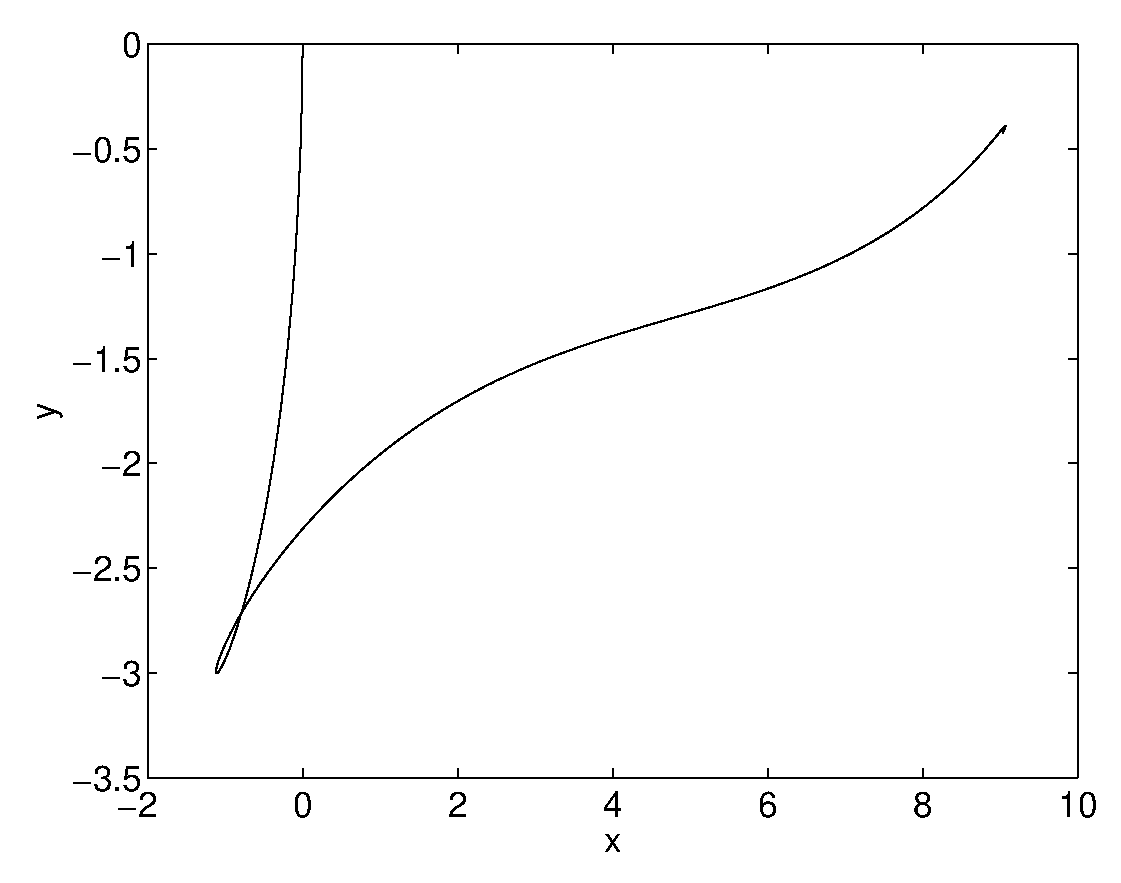
\includegraphics[width=\textwidth]{img/manip_task_path.eps}
\caption{path}
\end{subfigure}
~
\begin{subfigure}[b]{0.45\textwidth}
\centering
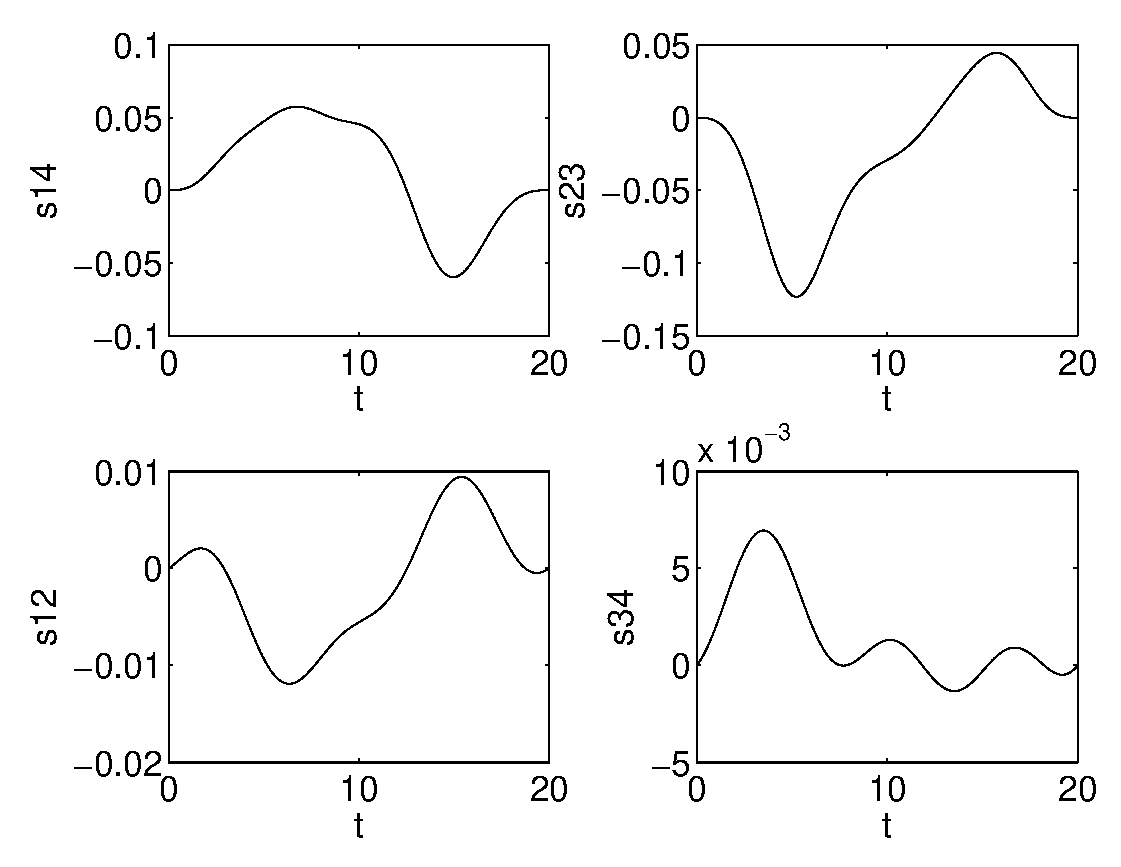
\includegraphics[width=\textwidth]{img/manip_task_slips.eps}
\caption{slips}
\end{subfigure}

\begin{subfigure}[b]{0.45\textwidth}
\centering
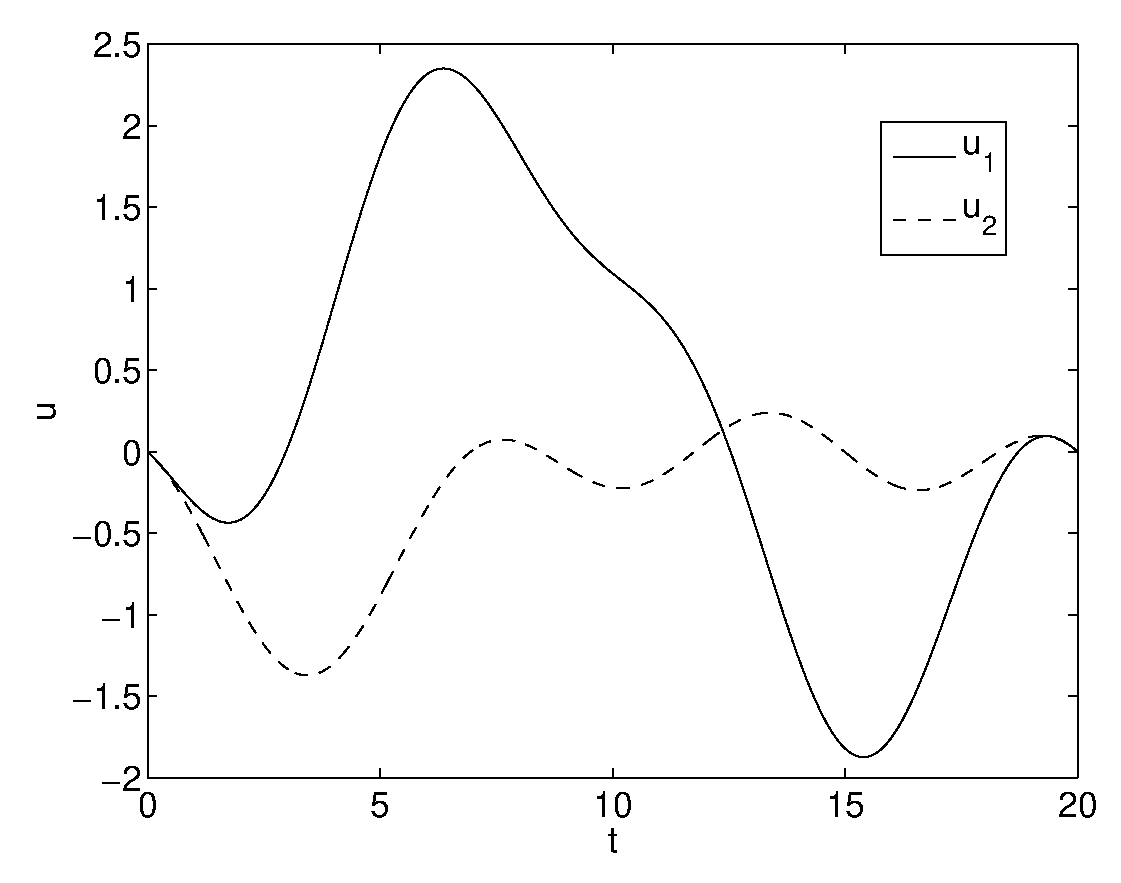
\includegraphics[width=\textwidth]{img/manip_task_u.eps}
\caption{control inputs}
\end{subfigure}
~
\begin{subfigure}[b]{0.45\textwidth}
\centering
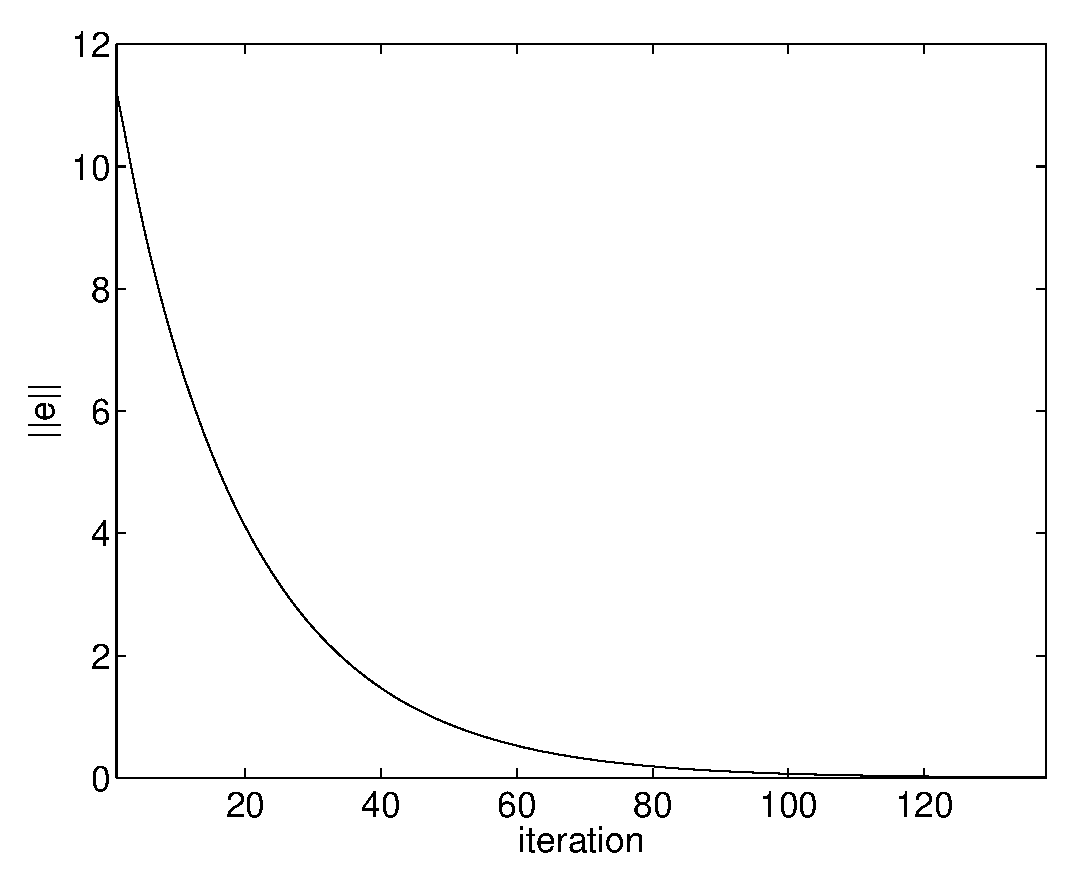
\includegraphics[width=\textwidth]{img/manip_task_err.eps}
\caption{error norm}
\end{subfigure}
\caption{Mobile manipulator, problem one}
\label{fig:pr1}
\end{figure}

\begin{figure}[h]
\begin{subfigure}[b]{0.45\textwidth}
\centering
\includegraphics[width=\textwidth]{img/manip_pltf_task_path.eps}
\caption{path}
\end{subfigure}
~
\begin{subfigure}[b]{0.45\textwidth}
\centering
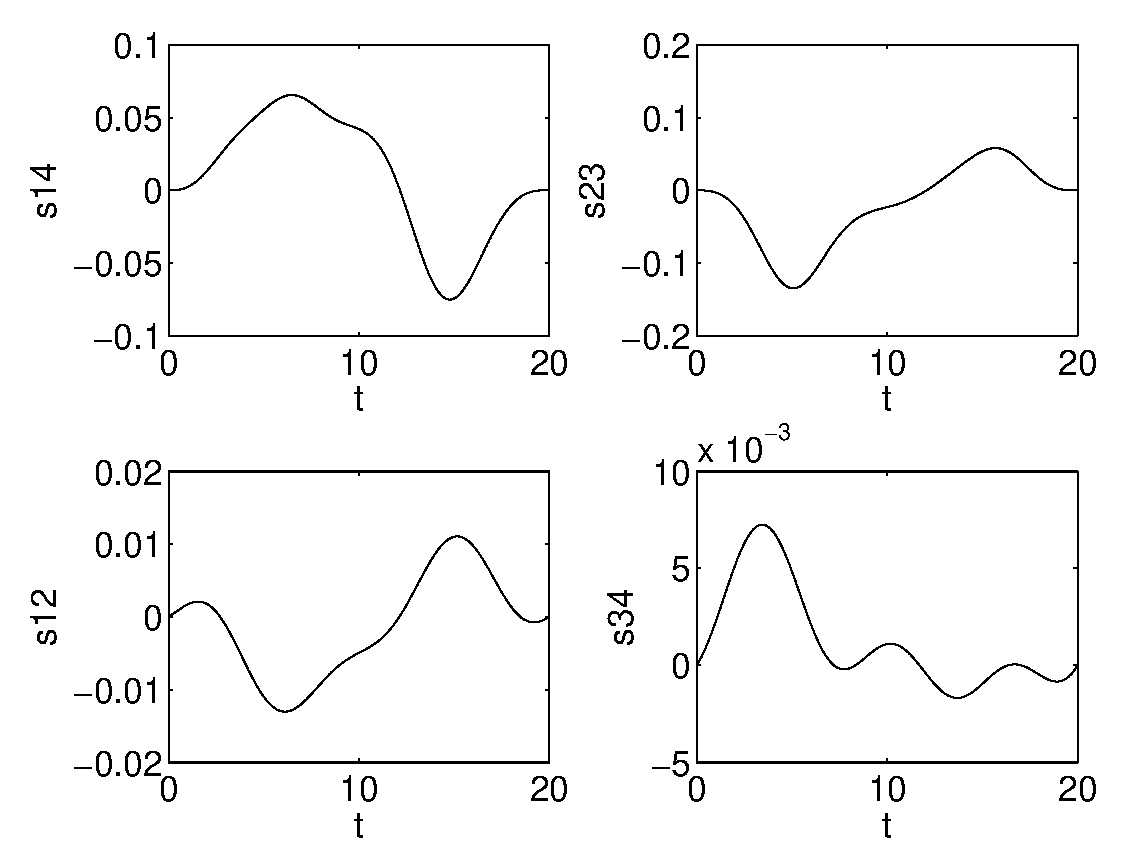
\includegraphics[width=\textwidth]{img/manip_pltf_task_slips.eps}
\caption{slips}
\end{subfigure}

\begin{subfigure}[b]{0.45\textwidth}
\centering
\includegraphics[width=\textwidth]{img/manip_pltf_task_u.eps}
\caption{control inputs}
\end{subfigure}
~
\begin{subfigure}[b]{0.45\textwidth}
\centering
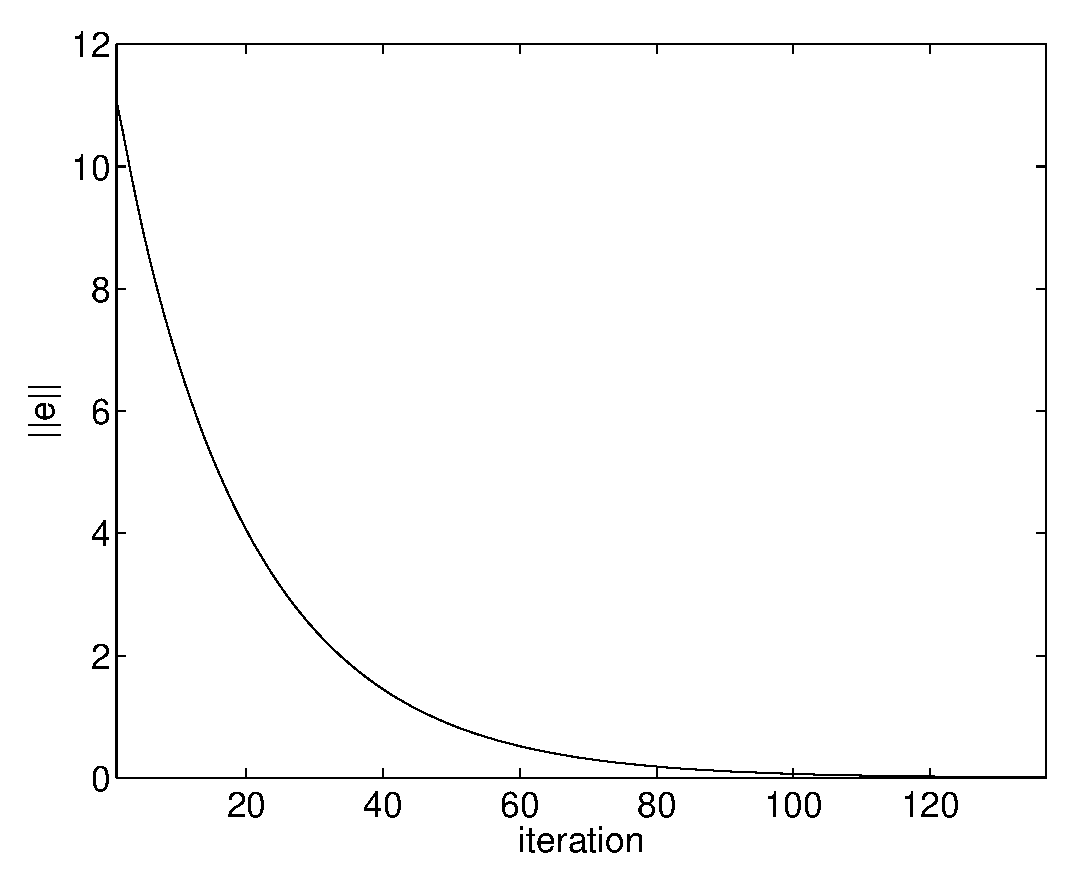
\includegraphics[width=\textwidth]{img/manip_pltf_task_err.eps}
\caption{error norm}
\end{subfigure}
\caption{Mobile manipulator, problem two}
\label{fig:pr2}
\end{figure}

\bibliography{library}
\bibliographystyle{unsrt}

\end{document}
%  LocalWords:  RTT
